\documentclass[10.5pt,listof=totoc]{report}  

\usepackage{chngcntr}
\usepackage{setspace}
\usepackage{graphicx}
\usepackage{float}
\usepackage[a4paper,left=30mm,right=30mm,top=30mm,bottom=30mm]{geometry}
\usepackage{etoolbox}
\usepackage[english]{babel}
\usepackage{array}
\usepackage{epigraph}
\usepackage{csquotes}
\usepackage{caption} 
\usepackage{multirow}
\usepackage{longtable}
\usepackage{xcolor,colortbl}
\usepackage{gensymb}
\usepackage{stmaryrd}
\usepackage{tcolorbox}
\usepackage{url}
\usepackage{adjustbox}
\usepackage{CJK}
\usepackage{lipsum}

\setcounter{secnumdepth}{3} % default value for 'report' class is "2"
\setcounter{tocdepth}{3}

% space between captions and tables
\captionsetup[table]{skip=10pt}

% double space paragraphs but not titles
\makeatletter
\pretocmd{\@chapter}{\singlespacing}{}{}
\pretocmd{\@sect}{\singlespacing}{}{}
\pretocmd{\@ssect}{\singlespacing}{}{}
\apptocmd{\@chapter}{\onehalfspacing}{}{}
\apptocmd{\@sect}{\onehalfspacing}{}{}
\apptocmd{\@ssect}{\onehalfspacing}{}{}
\makeatother
\onehalfspacing

% Define \tab
\newcommand\tab[1][6mm]{\hspace*{#1}}

% Change name "Contents" to "Table of Contents"
\addto\captionsenglish{\renewcommand{\contentsname}{Table of Contents}}


\begin{document}
\begin{CJK}{UTF8}{min}

\begin{titlepage}
	\centering
	
\includegraphics[width=0.4\linewidth]{Figures/eria.jpg}\par
	\vspace{5 cm}
	{\scshape\large Research Project Report\par}
	\vspace{0.4cm}
	{\LARGE \bfseries Integrated Space-based/Geospatial System to strengthen the Resilience and Connectivity of ASEAN\par}
	\vspace{3 cm}
	{\scshape\large Edited by\par}
	\vspace{0.4cm}
	{\large Prof.~Ryosuke \textsc{Shibasaki}, Prof.~Takayoshi \textsc{Fukuyo},\par}
	{\large Prof.~Hiroyuki \textsc{Miyazaki} and Mr.~Quentin \textsc{Verspieren}\par}
	\vspace{0.2cm}
	{\large \itshape The University of Tokyo\par}
	\vfill
	{\large October, 2017\par}
\end{titlepage}


\counterwithout{figure}{chapter}
\counterwithout{table}{chapter}

\pagenumbering{roman}

\cleardoublepage
% \phantomsection
\addcontentsline{toc}{chapter}{Foreword}
\chapter*{Foreword}

Today, space and geospatial technology (SGT) are no longer just fields of advanced technological development and scientific research, but they have become key component to help achieve sustainable development and strengthening resilience. They can improve the efficiency and resilience of industrial operations and effectively address issues in regional economic integration of  the ASEAN.

Based on this understanding, an ERIA study project "Applying Space-based Technology for building resilience in ASEAN region" was conducted in 2014 and concluded that geospatial technologies and space technologies have notable potentials to strengthen the resilience although sustainable mechanism for integrating the technologies  has not still been well established. The study pointed out necessity of (i) trans-border mechanism to deliver the geospatial and space-based information from data provider to end users in disaster-affected areas with support of international activities and (ii) financial schemes involving private sectors, or public-private partnerships (PPP), to operate collaborative integration of the technologies in sustainable and practical manners.

To implement such a mechanism, assessing the benefits from SGTs and applications and conceptualizing necessary policies are very important.
This report provides current status of SGT, applications, and potential benefits to the ASEAN based on the past practices in Asia and Pacific. It includes information about what technology and combinations of technologies were applied and how those contributes to resilience of ASEAN by key issues including urban development, infrastructure planning and management, transportation management, improving Quality of Life, post-disaster management, improving logistics efficiency, sustainable operations of agriculture and fishery, improving efficiency manufacturing and service industry, management of environmental services and natural resources.

Besides, This report covers policy perspectives with strategy options about how to implement the regional connectivity of ASEAN supported by the technologies, especially focusing on trans-border mechanism of data and information.

We hope that this report proves useful to the ASEAN, the participating states, and stakeholders who work with the ASEAN by guiding the SGT applications to the more connectivity of ASEAN states.

\begin{flushright}
\vspace{1 cm}
{\Large \bfseries Prof.~Ryosuke \textsc{Shibasaki}\par}
\vspace{0.2 cm}
{\itshape Professor, Center for Spatial Information Science\par}
{\itshape The University of Tokyo\par}
\end{flushright}


\cleardoublepage
% \phantomsection
\addcontentsline{toc}{chapter}{Project Members}
\chapter*{Project Members}

\begin{center}

{\large \bfseries Editor\par}

\vspace{0.3 cm}

{Prof.~Ryosuke \textsc{Shibasaki}\par}
{\footnotesize Professor, The University of Tokyo\par}

\vspace{0.8 cm}

{\large \bfseries Co-Editors\par}

\vspace{0.3 cm}

{Prof.~Takayoshi \textsc{Fukuyo}\par}
{\footnotesize Project Associate Professor, The University of Tokyo\par}
\vspace{0.2 cm}
{Mr.~Quentin \textsc{Verspieren}\par}
{\footnotesize Researcher, The University of Tokyo\par}

\vspace{0.8 cm}

{\large \bfseries Authors\par}

\vspace{0.3 cm}

{Prof.~Ryosuke \textsc{Shibasaki}\par}
{\footnotesize Professor, The University of Tokyo\par}
\vspace{0.2 cm}
{Prof.~Takayoshi \textsc{Fukuyo}\par}
{\footnotesize Project Associate Professor, The University of Tokyo\par}
\vspace{0.2 cm}
{Prof.~Hiroyuki \textsc{Miyazaki}\par}
{\footnotesize Project Assistant Professor, The University of Tokyo\par}
{\footnotesize Visiting Faculty, Asian Institute of Technology\par}
\vspace{0.2 cm}
{Mr.~Quentin \textsc{Verspieren}\par}
{\footnotesize Researcher, The University of Tokyo\par}

\vspace{0.8 cm}

{\large \bfseries Other members\par}

\vspace{0.3 cm}

{Mr.~Yoshinori \textsc{Kobayashi}\par}
{\footnotesize Japan Space Forum\par}

\end{center}

\cleardoublepage
% \phantomsection
\addcontentsline{toc}{chapter}{Acknowledgements}
\chapter*{Acknowledgements}

\tab The team acknowledges the organizational support of Susumu Yoshitomi, Takefumi Wakamatsu, Japan Space Forum; and Mayuko Saito, Nusantara Research Institute.

\vspace{0.4 cm}

For the time they gave us during this project's various interviews, the team would like to thank Thiri Maung, Ministry of Social Welfare, Relief and Resettlement, Myanmar; Sonephet Phosalath, Xailee Xayaxang, Phetsamone Dalalom, Bounteum Sysouphanthavong, Ministry of Natural Resources and Environment, Lao P.D.R.; Malyn Tumonong, Pimvadee Keaokiriya, Chandra Satriadi Putra, Tika Savitri Pandanwangi, Dimas Adekhrisna, ASEAN Secretariat; Munadjat Bambang, Fuadi Darwis, Susilastuti, Bambang, BNPB, Indonesia; Suryo Andri, AHA Centre; Tae Hyung Kim, Youjin Choe, UNESCAP; and Wasanchai Vongsantivanich, GISTDA.


\vspace{0.4 cm}

For their participation in the first workshop in Manila and their valuable inputs, the team would like to thank our various partners: Koji Saeki, Naoki Takarada, Cabinet Office of Japan; Koji Suzuji, National Research Institute for Earth Science and Disaster Resilience (NIED); Masanobu Tsuji, JAXA; Tadashi Sasagawa, PASCO; Peraya Tantianuparp, Hydro and Agro Informatics Institute (HAII); Masahiko Nagai, Yamaguchi University; Kazushi Motomura, RESTEC; I Nyoman Radiarta, Institute for Marine Research and Observation (IMRO), Indonesia; Osamu Kashimura, Japan Space Systems; Toshihiro Obata, The University of Tokyo; George Maeda, Pauline Faure, Kyushu Institute of Technology; Yuya Nakamura, AxelSpace; Mochamed Saleh Nugrahadi, Coordinating Ministry for Maritime Affairs, Indonesia; Agustan, BPPT, Indonesia; Abdul Rashid Mohamed Shariff, Universiti Putra Malaysia; Ariel C. Blanco, University of Philippines; Rogel Mari Sese, National SPACE Development Project, Philippines; Raweewan Nutpramoon, Raksina Lekthanoo, GISTDA; and Vu Tien Quang, Department of Survey and Mapping Viet Nam.

\vspace{0.4 cm}

Finally, for their participation in the second workshop in Jakarta, the team would like to thank Takashi Ikeda, Cabinet Office of Japan; Yuya Nakamura, AxelSpace; Oni Bibin Bintoro, Agustan, BPPT, Indonesia; Pimvadee Keaokiriya, ASEAN Secretariat; Fuadi Darwis, BNPB, Indonesia; Alvin Familara, National SPACE Development Program; in particular for their direct contribution to this report: I Nyoman Radiarta, Teja Arief Wibawa, Rizky Hanintyo, Komang Iwan Suniada, Institute for Marine Research and Observation (IMRO), Indonesia; M. Rokhis Khomarudin, Remote Sensing Application Center, LAPAN, Indonesia; Xaysomphone Souvannavong, Ministry of Natural Resources and Environment, Lao P.D.R.; Abdul Rashid Mohamed Shariff, Universiti Putra Malaysia; Thiri Maung, Ministry of Social Welfare, Relief and Resettlement, Myanmar; Adrian Josele G. Quional, National SPACE Development Program, Philippines; Jakrapong Tawala, GISTDA; and Vu Anh Tuan, Vietnam National Satellite Center.

\addcontentsline{toc}{chapter}{Table of Contents}
\tableofcontents

\cleardoublepage
% \phantomsection
\addcontentsline{toc}{chapter}{\listfigurename}
\listoffigures

\cleardoublepage
% \phantomsection
\addcontentsline{toc}{chapter}{\listtablename}
\listoftables

\addcontentsline{toc}{chapter}{List of Abbreviations}
\chapter*{List of Abbreviations}

\begin{longtable}{lp{12cm}}
\centering

{AADMER} & {ASEAN Agreement on Disaster Management and Emergency Response} \\
{ADB} & {Asian Development Bank} \\
{AHA Centre} & {ASEAN Humanitarian Assistance Centre} \\
{AI} & {Artificial Intelligence} \\
{ASCC} & {ASEAN Socio-Cultural Community} \\
{ASEAN} & {Association of Southeast Asian Nations} \\
{DDIE} & {Data-Driven Innovation Economy} \\
{DEM} & {Digital Elevation Model} \\
{DRM} & {Disaster Risk Management} \\
{ERIA} & {Economic Research Institute for ASEAN and East Asia} \\
{GHG} & {Greenhouse Gas} \\
{GIS} & {Geographic Information System} \\
{GISTDA} & {Geo-Informatics and Space Technology Development Agency} \\
{GNSS} & {Global Navigation Satellite Systems} \\
{GsMAP} & {Global Satellite Mapping of Precipitation} \\
{IMRO} & {Institute for Marine Research and Observation} \\
{IoT} & {Internet of Things} \\
{M2M} & {Machine to Machine} \\
{MPAC} & {Master Plan on ASEAN Connectivity} \\
{PDCA} & {Plan-Do-Check-Act} \\
{OECD} & {Organisation for Economic Co-operation and Development} \\
{QoL} & {Quality of Life} \\
{QZSS} & {Quasi-Zenith Satellite System} \\
{SGT} & {Space and Geospatial Technology} \\
{SMAC} & {Social-Mobile-Analytics-Cloud} \\
{UNESCAP} & {United Nations Economic and Social Commission for Asia and the Pacific} \\
{UNICEF} & {United Nations Children's Fund, previously United Nations International Children's Emergency Fund} \\
{WHO} & {World Health Organization} \\

\end{longtable}

\pagenumbering{arabic}
\addcontentsline{toc}{chapter}{Executive Summary}
\chapter*{Executive Summary}

Optimization of production processes is the most prioritized issues in the industrial factories. Such optimization is quite feasible because it is easy to acquire monitoring data  of environment and boundary conditions which are connected to productions. Besides, it is easy to project impacts of process changes. However, it is a challenge to extend the optimization beyond the factory processes, such as delivery to consumers and retail stock. It is  because factories do not have accesses to information on trends and amount of purchase and latency and incidents during cargo stowage and transport routes during delivery processes. These are actually uncertainties in optimization of the whole processes. For example, retails have to stock more than observed purchases for risks of unexpected latency of production and delivery while productions have to estimate longer periods for delivery than feasible periods due to uncertainties of incident occurrences.

Based on this, constructing large scale production systems by connecting variety of sectors like factory, delivery, and retail yields uncertainties between the connections and results in degradation of production efficiency.

Space and Geospatial Technology (SGT) had been developed as a intelligence technology. Space infrastructure, such as earth observation, positioning and tracking, and communications, helps more effective decision making to reduce uncertainty and risks by continuous monitoring and visualization of situational information of the real world, such as people mobility and activity, vehicle traffics, meteorology and oceanology,  and disaster.

Potentials of space infrastructure are rapidly growing along with the successes of small-scale and low-cost satellites. In addition, data infrastructure for big data and artificial intelligent technologies enables rapid integration and analysis of real world dynamics by variable data resources of earth observation and positioning and tracking from the space  infrastructure. SGTs support decision makers to swiftly monitor and accurately predict the situation and changes of people and companies. SGTs therefore facilitate more safety and less risk in decision making and activities by providing the dynamic situational information of general industry and people's lives.

For instance of heavy rain disasters, rapid areal monitoring flooded roads and traffic jams helps delivery services to response to reduce impact of service latency in the disaster situation by changing transports and routes. The reduction of uncertainty in delivery facilitate planning of production and retails with shorter production periods and less stocks.
Besides, SGT helps to record disaster responses as data which is useful for AI-based analysis to improve responses to future disasters.

This kind of SGT-based integration supports construction of large-scale production-delivery systems integrating many enterprises over various fields by reducing uncertainties caused by external factors. As the result, more various products and services are provided in more efficient manners.

In the ASEAN region, where many and various organizations and enterprises expand over large geographic extent and population, it is very important to proceed "unbundling" and "rebundling", with which communities and companies recognize their own roles and connect them over the ASEAN region, for the sustainable development. SGT should be an indispensable infrastructure of information sharing needed for the "unbundling" and "rebundling"

While the ASEAN prioritize to secure people's safety and stabilize living levels, SGT is also contributes to better resilience of the ASEAN region, which is the most populated and disaster-prone areas in the world, by providing proper dissemination and navigation against the disaster risks in their lives.

To proceed SGT-based integration in the ASEAN region, it is needed to promote public-private-partnership (PPP) of space infrastructure development and supporting ground infrastructure. Another important issue is establishing data policies facilitating trans-broader data transfer and utilization under proper management mechanism. This report provides recommendations about strategies and frameworks of ASEAN's data policy and space infrastructure development.

\chapter{Enhancing ASEAN connectivity through Space and Geospatial Technology} \label{enhancing}

\tab Space and Geospatial Technology (SGT) is an intelligence technology enabling the global monitoring of a wide range of parameters such as the distribution of facilities and buildings, the movements of cars, ships, aircrafts, and people, environmental change, or post-disaster economic development processes. While geospatial technology was originally developed for military and security use, it has been,in recent years, quickly advanced towards an utilization as a \textbf{general consumer technology}. It is now widely applied in the field of public services (e.g. disaster response, social infrastructure management, traffic management), business support (e.g. marketing), and personal mobility services (e.g. navigation). The extensive use of low-cost and high-performance mobile devices --- such as smart-phones --- has further accelerated its popularization all over the world. Later, the development of \textit{Internet of Things} (IoT) and \textit{Artificial Intelligence} (AI) technologies enabled researchers to conduct \textbf{deeper analyses and information collection}. In this regard, geospatial technology has been expected to expand much further its utilization and development in the future.

\vspace{0.4 cm}

This chapter will be organized as follows:

\begin{enumerate}

\item Define and introduce generally the potential of SGT in various fields.

\item Present the original application of SGT (disaster management) and its wider potential for economic strengthening.

\item Finally, develop more concrete consideration on the use of SGT and data sharing to advance towards an data driven ASEAN.

\end{enumerate}


\section{The immense potential of Space and Geospatial Technology}

\tab This section aims at introducing the concept of SGT and at briefly presenting general applications of SGT.

\subsection{What is SGT?} \label{wi_sgt}

The rise of intelligence technologies resulted in the development of three different technological areas of \textbf{space infrastructure}: 

\begin{itemize}

\item \textbf{Satellite-based earth observation technology}, monitoring occurrences all over the world.

\item \textbf{Positioning technology}, measuring precise positions in real time.

\item And \textbf{communication technology} to connect almost instantly every single part of the world.

\end{itemize}

The most important application of space infrastructure (observation, positioning and communication) is what is called \textbf{Geospatial Technology}. Geospatial technology can be seen as a global information technology, providing services anywhere in the world based on space infrastructure, as illustrated on figure \ref{sgt}. Therefore, the improvement of the performances of space infrastructure directly leads to the improvement of the performances of geospatial services. It is then primordial to simultaneously advance the development, maintenance, and use of both of these technologies. What is called \textbf{Space and Geospatial Technology (SGT) is the combination of space infrastructure with geospatial technology}, which constitutes the core of this report.
 
\begin{figure}[H]
\begin{center}
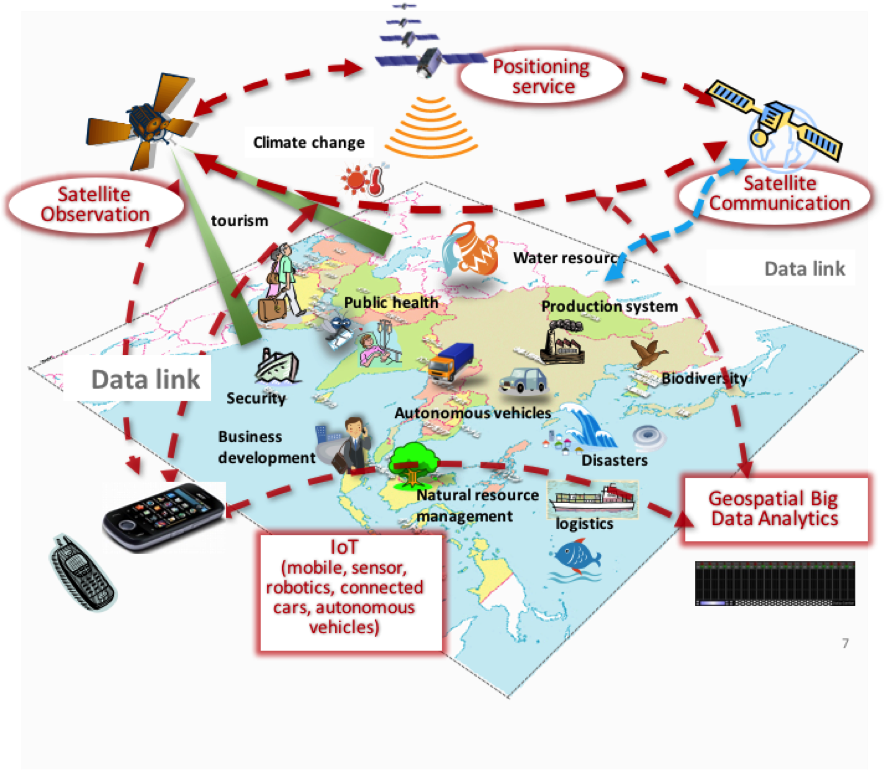
\includegraphics[width = 0.8\linewidth]{Figures/sgt.png}
\end{center}
\caption{Space infrastructure and technologies supporting SGT}
\label{sgt}
\end{figure}

More concretely, SGT consists of four aspects:

\begin{enumerate}

\item \textbf{Real-time location and trajectory} of people, cargo and vehicles (air, sea, and land).

\item \textbf{Real-time environmental and contextual information} covering all land and sea, such as: dynamic maps (traffic, congestion, people flow, and city changes) or environmental changes (weather, water and air quality, and greenery) from which events, accidents, and disasters can be extracted. Silent but meaningful changes such as crustal deformation can be included.

\item \textbf{"Ubiquitous" data communications} at anytime/anywhere with small IoT devices to collect data from and to send instructions/guidance to people and machines in the field.

\item \textbf{High precision mapping} for autonomous vehicles and machines and crust movement monitoring.

\end{enumerate}


\vspace{0.4 cm}

\textbf{Satellite observation is extremely flexible} compared with airborne observation performed by aircraft or drones which suffers from airspace restriction, small coverage, and limited flight time. \textbf{Real-time positioning by satellites can be performed by compact and inexpensive portable terminals}, currently installed in almost all smart-phones as well as in most vehicles, airplanes, or ships. Therefore, the mobility data of people, vehicles, ships, and aircraft are widely available.

\vspace{0.4 cm}

Geostationary satellites are commonly used for data communication. However, the sufficient \textbf{miniaturization of ground transceivers combined with the use of the low earth orbit satellites constellation} will increase the access to efficient communication and dramatically reduce costs in a near future. Therefore, data communication will be available everywhere, as long as the sky is visible. 


\subsection{Generic examples of SGT application}

\tab Such a technological environment can be simultaneously established all over the world, allowing the promotion of several services using space infrastructures in various countries and regions. 

For instance, small portable terminals equipped with Global Navigation Satellite Systems (GNSS) receivers are commonly distributed on land and sea, such as smart-phones, now widely distributed in most countries around the world. Also, the use of \textit{black boxes} --- a device combining a GNSS receiver with a communication system, constantly transmitting its localization --- in most ships and aircraft improved locational information collection of commercial vehicles. Finally, the development of IoT (Internet of Things) has allowed the collection of data from large systems composed of various sensors.

As described earlier, the use of space infrastructure enables to understand the movement of people, vehicles, and cargos. Furthermore, satellite imagery analysis helps to visualize the reasons of people behavioral changes such as traffic congestion, disaster situations, construction of buildings and infrastructure, and change of agricultural land.

\vspace{0.4 cm}

While the easy gathering of production-related information in factories has greatly contributed to the optimization of production processes in industrial activities, the collection of information related to external environment changes --- such as traffic, people flow, and logistics --- was hard to obtain. Therefore, SGT can help providing this kind of information, in order to facilitate closer cooperation between various actors of the service and manufacturing sectors. 

\vspace{0.4 cm}

Finally, for actors mostly involved outdoor tasks such as construction, agriculture, fishery, and forestry, SGT allows to obtain very accurate locational information for further optimization.

\section{The various roles of SGT}

The original target for the general civil application of SGT was disaster response. Based on an extensive number of previous studies and famous achievements in this field, it has been confirmed that SGT can be applied to the strengthening of the socioeconomic system and the development of efficient Disaster Risk Management (DRM) in the Association of Southeast Asia Nations (ASEAN).

\vspace{0.4 cm}

In this section, we first examine the use of the SGT in the field of DRM before discussing more generally the importance of data sharing in ASEAN countries.

\subsection{SGT for disaster management in ASEAN}

\tab The Asia-Pacific region, most populated region on Earth with more than 4.5 billion souls, is also the daily theater of the planet's deadliest disasters. From typhoons to earthquakes, from tsunamis to volcanic eruptions, the region's countries suffer from tremendous consequences for their population, their economy and their environment, trapping them in a vicious circle of increasing vulnerability. 

The strong impact of disasters in the Asia-Pacific region does not simply rely on the intensity of these unfortunate events but also on a set of systemic weaknesses of Asian countries: economic and financial fragility, galloping urbanization, exploding demography or lack of land use planning.

\vspace{0.4 cm}

One of the main reasons of the vulnerability of the Asia-Pacific region to disasters is its demography. Asia-Pacific is the most populated area in the world with more than 4.5 billion inhabitants in 2016 according to the United Nations Economic and Social Commission for Asia and the Pacific (UNESCAP) \cite{PopulationDataSheet}. In the region can be found most of the world's largest metropolises. In 2016, the United Nations estimated that 18 of the world's 31 megacities (more than 10 million inhabitants) were located in Asia-Pacific and that this number is expected to reach 24 out of 41 in 2030 \cite{WorldCities}. These high densities of population often located around riverside flood areas, along coastlines at risk of tsunami or at the base of landslide-prone mountains put large numbers of human life in jeopardy.

\vspace{0.4 cm}

In its 2015 Asia-Pacific Disaster Report, the UNESCAP dresses a sad portrait of the region. Between 2005 and 2014, 1,625 incidents had been reported. Most of these disasters were floods, followed, in order, by storms, earthquakes and tsunamis and landslides.

These disasters had a dramatic impact on the region's human security by killing almost half-a-million inhabitants in Asia-Pacific and were directly affecting the lives of approximately 1.4 billion people (see table \ref{HumanLossAP}). Moreover, beyond long term economic impact due to the loss of workforce as well as the increase of spending for health related issues, the 1,625 disasters evoked in the previous paragraph generated direct economic damages worth \$523 billion. 

\begin{table}[h]
   \caption{\label{HumanLossAP} Human impact of disasters in Asia and the Pacific, total 2005-2014 \cite{APdisaster2015}}
   \centering
   \begin{tabular}{| >{\columncolor[gray]{.9}}l | c | c |}
   \hline
     \rowcolor[gray]{.8}
     Disaster type & {Lives lost} & {People affected (millions)} \\
   \hline
    Earthquakes and tsunamis & 199,418 & 74 \\
    Storms & 166,762 & 321 \\
    Floods & 43,800 & 771 \\
    Others & 73,772 & 199 \\
   \hline  
    Total & 483,752 & 1,366 \\
   \hline   
   \end{tabular}
\end{table}

Finally, the UNESCAP report stresses the fact that although these numbers are impressive, they may be underestimated due to a lack of serious disaster data gathering initiative \cite{APdisaster2015}.

\vspace{0.4 cm}

Beyond natural disasters, strengthening food and water security is a priority for the development organisations operating in the region. According to an ADB report on food security, in 2010, more than 700 million people in Asia-Pacific survived with less than \$1.25 per day, in an environment where high and volatile food prices cause 537 million of them to suffer from hunger (62\% of the world) \cite{ADBfood}. Moreover, as 80\% of water resources are still exclusively used for agriculture, the region is particularly affected by water insecurity: 1.7 billion people do not have access to basic sanitation, 80\% of wastewater is directly dumped into rivers, lakes or seas with almost no treatment \cite{AWDO2016}. In terms of economic development, it is estimated that the annual global cost of water insecurity reaches \$500 billion, corresponding to a loss of more than 1\% global gross domestic product \cite{sadoff}. It goes without saying that the dramatic advance and intensification of climate change will considerably amplify all these issues as well as many others including water level increase, desertification, scarcity of available water resources, climate refugees migrations or the intensification of large scale meteorological disasters. Finally, UNICEF recently raised an alarm about the increasing dangers posed by air-pollution. According to the UN agency's data, more than two billion children live in areas where outdoor air-pollution levels exceed WHO guidelines, including 1.07 billion in Asia-Pacific. Moreover, air pollution kills 600,000 children under five yearly.

\vspace{0.4 cm}

It is therefore primordial for ASEAN to develop and implement ambitious disaster risk management policies. In this regards, SGT and more generally data sharing can play a prominent role, as clearly stated in the \textit{AADMER Work Programme 2016-2020} \cite{aadmer_wp}:

\begin{displayquote}

Promote regional standards, including methodologies and tools to assess, record, calculate the disaster losses and damages, and share non-sensitive data and create common information system, to enhance interoperability, ensure unity of action, and strengthen resilience.

\end{displayquote}

However, the maintenance costs of such a large infrastructure as data sharing are extremely high. It should therefore be smartly and strongly designed, not only for disaster management but for multi-purpose usage, aiming at the strengthening of the regional  socioeconomic environment. Furthermore, beyond the impact of the system, it should be made in an economically sustainable way, which is a significant challenge.


\subsection{SGT for economic strengthening through enhanced connectivity} \label{enhanced}

As explained above, the potential of SGT incites users to go further than immediate issues related to disaster management by using it as an ambitious tool, at all level of the economy.

\vspace{0.4 cm}

SGT largely contributes to decision-making processes among governments, companies, communities, cities, individuals in various contexts by providing necessary information. As SGT enhances the economy and facilitates \textit{'smartification'} across borders, it is extremely effective to connect all actors of ASEAN. Therefore, this study examines possible contributions of SGT system infrastructure to strengthen ASEAN connectivity.

\vspace{0.4 cm}

Furthermore, strengthening ASEAN connectivity is also essential for cross-border utilization of SGT. Therefore, the study also provides policy recommendations aiming at the enhancement of ASEAN connectivity, in order to maximize the use of SGT.

\begin{figure}[H]
\begin{center}
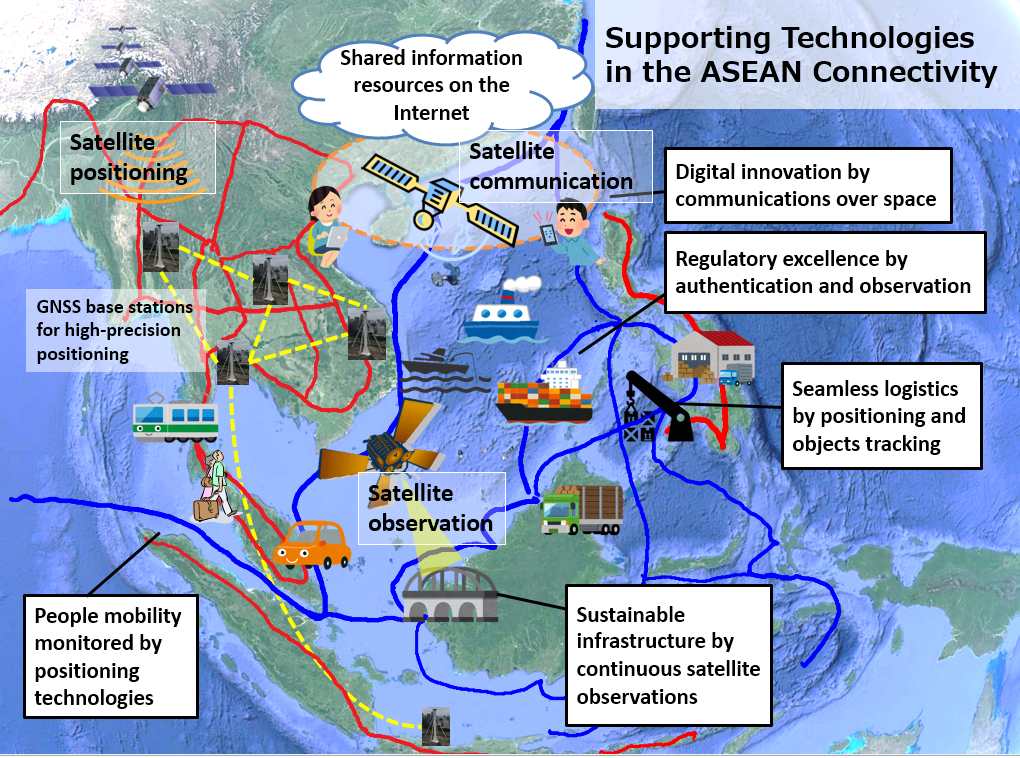
\includegraphics[width = 0.8\linewidth]{Figures/supp_connect.png}
\end{center}
\caption{Supporting technologies in the ASEAN connectivity}
\label{supp_connect}
\end{figure}

{\flushleft \bfseries Therefore, this study addresses:\par}
\vspace{0.2 cm}
{\bfseries A common platform and infrastructure of Space \& Geospatial Technology for DRM to enhance ASEAN connectivity and realize human development, resiliency, and sustainable development. The sustainability of the system will reside in its value-creation process\par}

\vspace{0.4 cm}

The approach of this study is perfectly in line with the ambitious \textit{Master Plan on ASEAN Connectivity 2025} or \textit{MPAC-2025} \cite{mpac}. Adopted in 2016, it targets the following sectors as main contributors to ASEAN Connectivity Strategies: Sustainable Infrastructure, Digital Innovation, Seamless Logistics, Regulatory Excellency, and People Mobility. SGT can contribute to these strategies, by being advantageously utilized for addressing common issues, developing common interests, and creating common infrastructures.

\vspace{0.4 cm}

In addition, SGT is expected, in the \textit{ASEAN Socio-Cultural Community Blueprint 2025} (ASCCB-2025) \cite{asccb}, to contribute to make ASEAN more:

\begin{itemize}
\item \textbf{Sustainable} through its application on biodiversity conservation, climate change, urbanization, production, and consumption.
\item \textbf{Resilient} through disaster response and health care. 
\item \textbf{Dynamic} through science and technology development.
\end{itemize}

These strategies and solutions can be efficiently expanded to the entire ASEAN region thanks to the extensiveness, the immediacy and the transboundary nature of space technologies.

\vspace{0.4 cm}

Specifically, while levels of ground infrastructure maintenance greatly vary with the degree of economic development, space system can provide the same information and services to the whole region. Therefore, strategies and good practices obtained from the MPAC-2025 and the ASCCB-2025 can be freely applied to ASEAN countries by overcoming national infrastructural limitations.


\section{Towards a data-driven ASEAN}

\tab At the end of 2015, the OECD published a major report entitled \textit{Data-Driven Innovation -- Big Data for Growth and Well-Being}. It states that \textit{'digitalization'} and data conversion of various activities will be advanced innovations, and a new economy will be developed accordingly \cite{oecd_ddi}.

The existing various common infrastructures (communication and meteorological satellites) and traditionally dynamic interactions (trade, information sharing, and interaction) in the ASEAN region makes it the perfect place for the emergence of upgraded version of data-driven innovation economy (DDIE). In particular, by removing physical restrictions, SGT will support ASEAN transformation into a DDIE 2.0.

\begin{figure}[H]
\begin{center}
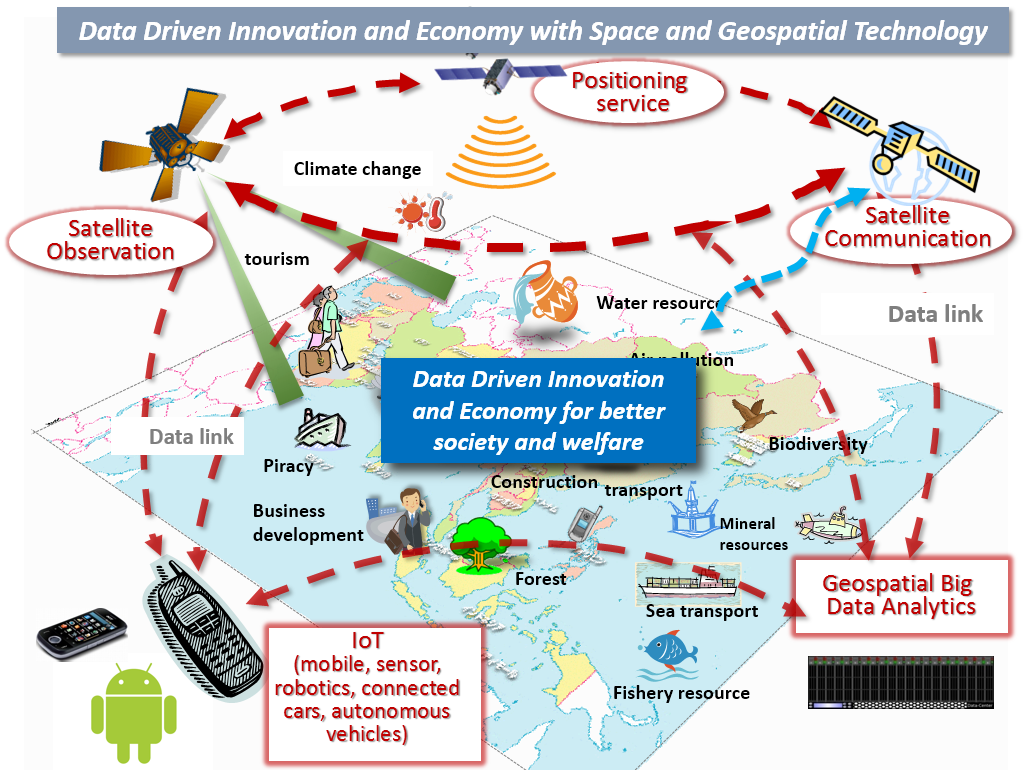
\includegraphics[width = 0.8\linewidth]{Figures/data_driven.png}
\end{center}
\caption{Data driven society through SGT}
\label{data_driven}
\end{figure}

\subsection{The tremendous economic potential of SGT}

\tab To understand more the prominent role that could be played by SGT in promoting innovation in ASEAN, let us look again at the MPAC-2025 \cite{mpac}. In its focus on digital innovation, it claims that:

\begin{displayquote}

Disruptive technologies (particularly mobile Internet, big data, cloud technology, the Internet of Things, the automation of knowledge work and the Social-Mobile-Analytics-Cloud or SMAC) could unleash some \$220 billion to \$625 billion in annual economic impact in ASEAN by 2030.

\end{displayquote}

In other words, it is SGT that will help to unleash these hundreds of billion USD, which may be derived from increased efficiency, new products and services, etc.

\subsection{From local to global optimization} \label{optimization}

As briefly explained above, one of the greatest strengths of SGT is its capacity to go beyond local optimization --- at factory level --- to achieve global optimization --- taking into account external factors and interrelations.

\vspace{0.4 cm}

The use of digital technology for monitoring and control within factories is already well developed, allowing an optimal use of resources and means of production.

However, information such as logistics between the factory and its partners (distributing networks, providers, etc.) is very insufficient. Any logistical irregularity will impact the whole production system, independently from the quality of the local optimization within the factory.

\begin{figure}[H]
\begin{center}
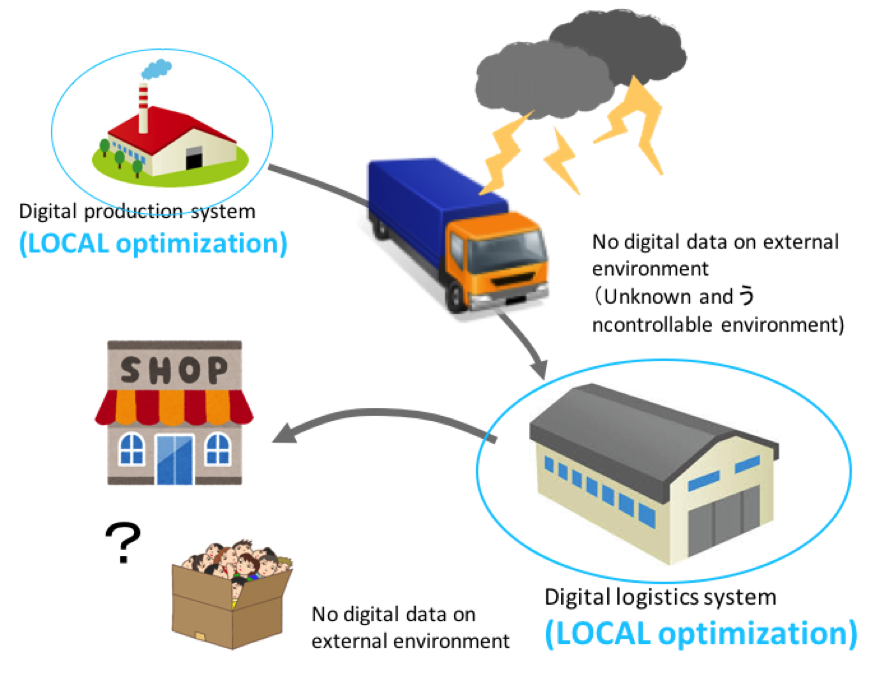
\includegraphics[width = 0.7\linewidth]{Figures/local_optimization.png}
\end{center}
\caption{Local optimization}
\label{local_optimization}
\end{figure}

Therefore, changes in the external environment can be major risks when data cannot be obtained, showing the limits of local optimization, as described on figure \ref{local_optimization}. While external environment cannot be directly controlled, if real-time data can be obtained, the production system can be adapted to the changes and risks can be significantly reduced.

Furthermore, in sector organized around outdoor activities, such as in construction, agriculture, forestry and fishery industries, sufficient information required for the production cannot be easily obtained. 

\vspace{0.4 cm}

SGT seamlessly digitalizes all spaces including external environments. It is therefore possible to optimize the entire system by considering external environmental changes. Figure \ref{global_optimization} expresses this idea.

\begin{figure}[H]
\begin{center}
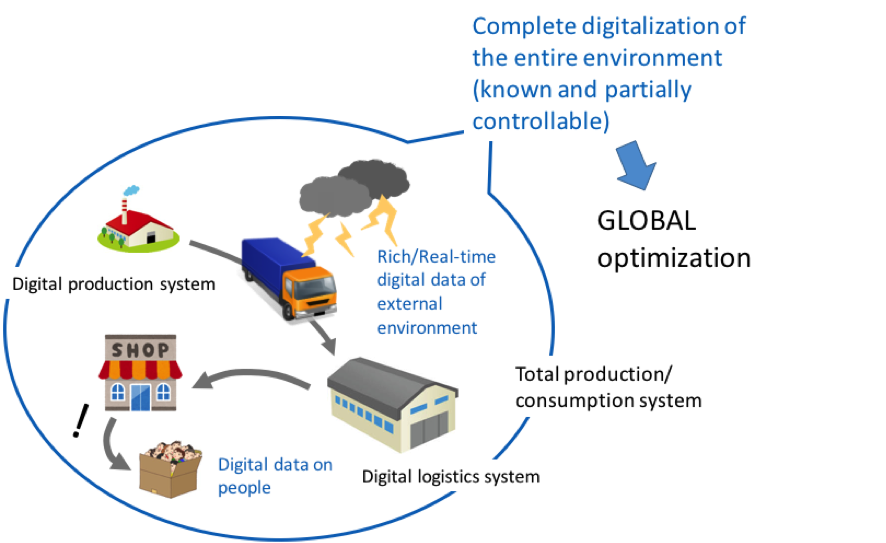
\includegraphics[width = 0.8\linewidth]{Figures/global_optimization.png}
\end{center}
\caption{Global optimization}
\label{global_optimization}
\end{figure}


\subsection{Achieving the third unbundling} \label{unbundling_p}

\tab In the current ASEAN situation, without widespread SGT applications, the optimization process of the whole production system connecting companies is extremely complicated as external environment is largely unknown. As a result, companies try to optimize their own production as much as possible by incorporated into a single organization (factory) all productive actors, hence, drastically reducing unbundling. Figure \ref{unbundling} shows the concept of unbundling in production and industrial systems.

\begin{figure}[H]
\begin{center}
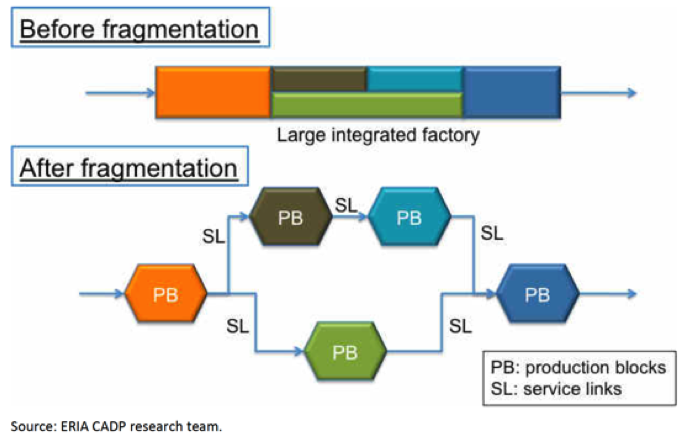
\includegraphics[width = 0.8\linewidth]{Figures/unbundling.png}
\end{center}
\caption{The concept of unbundling}
\label{unbundling}
\end{figure}

However, if sufficient digital data on external environment are obtained, it is possible to control the whole production system for optimization by incorporating the external changes. As a result, it is not required to build up each component of a production system in the company. Unbundling of the production system can be advanced to a large scale.

\vspace{0.4 cm}

While a change in logistics thanks to SGT accelerates the 2nd unbundling --- spatial separation of production blocks, it is expected that the spatial separation of engineers and managers involved in the production will also be further accelerated. This \textbf{3rd unbundling} will be achieved through the digitalization of production systems that is to say the digitalization of people, goods, and real-time monitoring.


\subsection{Conclusion: Enhancing ASEAN digitalization and connectivity with SGT}

In summary, Data Driven Innovation as proposed by the OECD is a general concept stating that industrial innovation will be developed through data utilization.

On the other hand, SGT effectively facilitates the optimization of the whole economic system --- production, consumption, services, etc. --- by digitalizing the external environment of individual production and business activities. 

\vspace{0.4 cm}

In ASEAN, where sudden external environmental changes, such as disasters, frequently occur, DDIE associated with SGT plays a significant role. Understanding such changes is not only important for the optimization of production systems but is also essential for improving social welfare including life stability and safety of local populations.

It can therefore be said that SGT will rapidly strengthen the inter-connectivity of ASEAN countries. As a result, it will strongly support industrial innovation, economic advancement, and social welfare.

\vspace{0.4 cm}

{\bfseries In short, Space \& Geospatial Technologies will create immense value through the realization of Data-Driven Innovation and Economy 2.0 and the Third Unbundling in ASEAN.}






















\chapter{Innovative SGT for the ASEAN economy}


\tab Following general considerations on the potential of SGT in chapter \ref{enhancing}, this chapter will present concrete areas of application of SGT in ASEAN. 

\vspace{0.4 cm}

This chapter will be divided in the following section:

\begin{enumerate}

\item A reminder of the general role and potential of SGT.

\item The presentation of key areas of application of SGT for ASEAN economy.

\item Finally, concrete recommendations based on the key areas introduced in section 2.

\end{enumerate}


\section{The role of SGT}

\tab As described in the previous section, SGT consists of four aspects:

\begin{enumerate}

\item Real-time location and trajectory of people, cargo and vehicles (air, sea, and land) in mass.

\item Real-time environmental and contextual information covering all land and sea, such as: Dynamic maps (traffic, congestions, people flow, and city changes), Environmental changes (weather, water and air quality, and greeneries) from which events, accidents, and disasters can be extracted. Silent but meaningful change such as crustal deformation can be included.

\item Supported with “Ubiquitous” data communications at anytime/anywhere with; Small IoT devices to collect data from and to send instructions/guidance to people and machines in the field.

\item High precision mapping, autonomous vehicles, and machines, crust movement monitoring

\end{enumerate}

For 1, it is technically possible to track most of all locational information of cars and people with the use of the wide-distributed smartphones. Relating 4, Quasi-Zenith Satellite will start its full operation in 2018, and seven aircraft will be operated in 2023. Along with these developments, reinforcement service such as MADOCCA will be provided; and more accurate location information can be obtained. As a result, location information can be rapidly applied in various fields such as automatic driving and track of ground movement. Regarding 3, an integration of various information covering people and cars in mega cities, and interior areas including oceans and rural communities can be achieved resulting in IoT sensor networks and M2M communication networks developments. Indeed, Oneweb will provide a network on the whole earth by 20XX, and its implementation will be started by 2025. About 2, based on the PLANET and AXELGLOB plans, real-time monitoring of the entire globe can be operated in 2025.

\vspace{0.4 cm}

These four principal functions are supposed to be implemented by 2025. Therefore, as described in the previous section, it is necessary to discuss the 2025 infrastructure strategy indicated by the MPAC, and its sustainability, toughness, and innovation of the ASCC blueprint associated with the current technological innovations.

\vspace{0.4 cm}

The following figure explains the overall concept of SGT.

\vspace{0.4 cm}

\begin{figure}[H]
\begin{center}
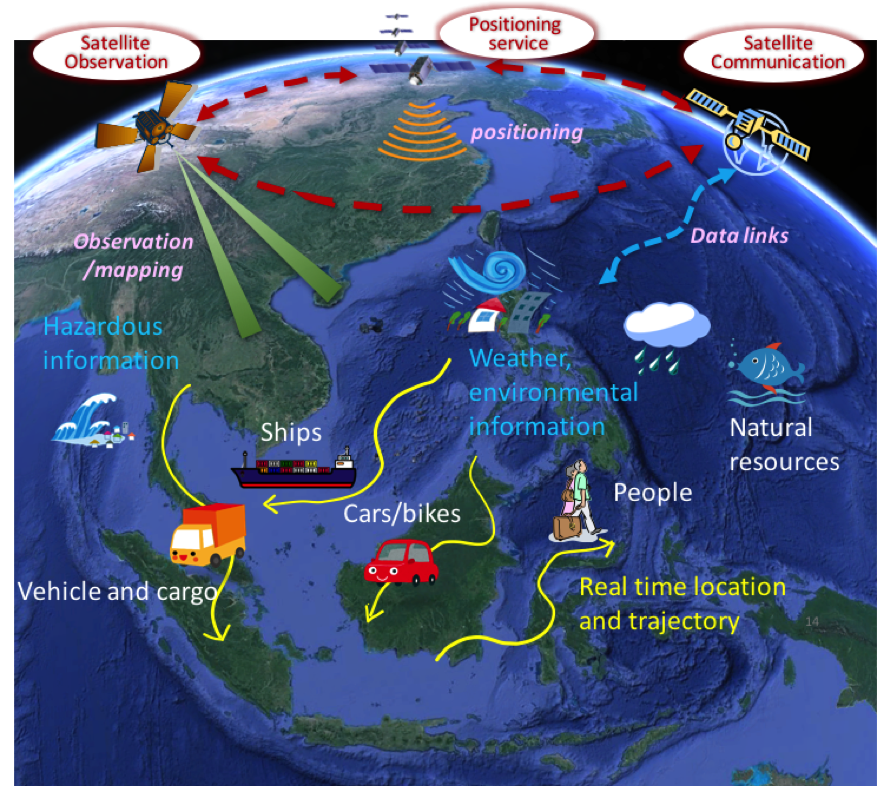
\includegraphics[width = 0.8\linewidth]{Figures/sgt_overall.png}
\end{center}
\caption{Overall concept of SGT}
\label{sgt_overall}
\end{figure}

\vspace{0.4 cm}

There are many common challenges in the ASEAN countries. For example, economic development and population growth are remarkable. Furthermore, there is a great potential for socio-economic developments resulting in excellent human resources developments. On the other hand, shortage of infrastructure investments, traffic congestion, environmental destruction, urban problems, and income disparity has been severely deepened.

\vspace{0.4 cm}

On the other hand, risks of natural disasters such as storms, floods, earthquakes, tsunamis, and landslides are high; therefore, a huge investment is required for proper disaster managements. Transportation network developments connecting each country and socioeconomic developments cooperated by countries are still insufficient.

\vspace{0.4 cm}

SGT provides essential information for disaster response, expansion, and strength of international transportation networks, reduction of traffic congestion, optimization of logistic, comprehensive urban management, and strengthens the PDCA cycle.




\section{The great potential of SGT}

The solutions associated with basic infrastructure and technology of SGT are as follows.

\begin{enumerate}

\item Better Urban Development/Control including more sound financial basis
\item Better infrastructure plan and management incl. financing \item Better and safer, smoother Transportation Systems
\item Better Quality of Life by reducing cost and risks from disaster, accidents and diseases, and increasing job and financing opportunities.
\item Better Disaster Responses, Evacuation, and Recovery.
\item More efficient and secure Logistics.
\item More stable and profitable, safer and sustainable agriculture and fishery while conserving resources and environment
\item More efficient manufacturing and service industries supported by better logistics and micro-financing.
\item Better quantification and management of environmental services and national resources.

\end{enumerate}

\subsection{Better Urban Development/Control including more sound financial basis}

\tab Information such as stagnation and movement of people and vehicles, urban facilities developments, construction of houses, and infrastructures such as roads can be continuously provided by SGT; therefore, government and local communities can conduct proper policy making and monitoring aiming for urban planning, urban growth management and environmental improvement in an efficient way. For example, individual information on stagnation and movement condition of people and vehicles can be used for introducing new taxes such as congestion billing and space use charge. Furthermore, extraction of building and land use from satellite imagery can be utilized for strengthening building taxation, and land tax levies. To apply location information for taxation, it is necessary to implement a location authentication system to prevent spoofing.

\subsection{Better infrastructure plan and management incl. financing (road pricing etc.)}

\tab Infrastructural conditions can be timely detected through image analysis and sensor information; therefore, it contributes to preventing accidents caused by infrastructure damages and further to optimizing maintenance methods and timing of infrastructure. Real-time digital data of vehicles and people using transport infrastructure helps to improving optimization of infrastructure investment, and the overall optimization of infrastructure management. For instance, an infrastructure usage-based charging system can be newly applicable; as a result, new resources and budgets for infrastructure management can be secured. To apply location information for taxation, it is necessary to implement a location authentication system to prevent spoofing.

Similarly, real-time supply and consumption of energy infrastructure can be obtained as digital data; it also contributes to optimizing infrastructure investment, and overall optimization. Particularly in the field of renewable energy, more detailed and reliable data on natural environments can be obtained by SGT; therefore, it contributes to optimizing its location and power transmission.

\subsection{Better and safer, smoother Transportation Systems}

\tab In the transportation system, SGT can track locations of vehicles, passengers, and cargo; therefore, it helps to real-time performance monitoring of transportation systems (smoothness, efficiency, and safety). SGT easily detects problems and continuously improves optimization of the scheme. Furthermore, automatic operation and sharing of vehicles can be performed by using real-time positioning service, which dramatically improves efficiency and smoothness of the transportation system. Further, it provides a possibility to simultaneously improve uneconomical external factors such as traffic congestion, air pollution/noise, Greenhouse Gas (GHG) emissions. Also, improvements of traffic congestion greatly contribute to the improvement of productivities (e.g., service industry) by shortening traveling time in cities. Moreover, freedom of location (houses and shops) in towns can be significantly improved, enabling city expansion and improving competitiveness. To secure the safety of automatic operation, improvement of the security of positioning service is necessary.

\subsection{Better Quality of Life by reducing cost and risks from disaster, accidents, and diseases, and increasing job and financing opportunities}

\tab Collection and provision of real-time disaster information by SGT efficiently helps to reduce disaster risks. It significantly contributes to improving Quality of Life (QoL) in Asia where disasters generate huge victims. Also, risks information such as traffic accidents and diseases can be provided as a temporal/spatial distribution so that these risks can be effectively reduced. Furthermore, collecting credit information for micro credit is available, providing an evidence of individual mobility pattern data This system contributes to increasing employment opportunities, such as matching for temporary work. Also, the quality of life among people in terms of safety and income can be continuously traced and evaluated so that continuous improvement can be carried out through the PDCA cycle.

\subsection{Better Disaster Response, Evacuation and Recovery}

\tab The use of SGT helps to quickly and exhaustively detect hazardous areas during disasters such as floods, landslides, earthquakes, and tsunamis. Therefore, evacuation can be promptly carried out in zones with a high level of risk, leading to the reduction of possible damages. Moreover, the knowledge of the distribution and condition of evacuees facilitates the efficient provision of medical services and distribution of necessary items to the victims.

Furthermore, SGT allows to monitor post-disaster activities such as rebuilding or economic recovery of damaged areas. By performing continuous and detailed assessments of disaster response and recovery activities, it helps to provide in a timely manner appropriate support at suitable stages. Furthermore, problems can be continuously discovered and solved through the PDCA cycle.

\subsection{More efficient and secure Logistics}

\tab The use of SGT enables to track movements of cargo, transportation vehicles and ships in real-time so that a reliable and continuous evaluation of transport performances can be made, leading to a significant reduction of the cost and duration of transportation.

Beyond this basic aspects, several points can be improved by using SGT:

\begin{itemize}

\item 

\end{itemize}
In case of disasters and failures, logistical delays can be forecast; therefore, damages can be reduced by adapting production amount and its distribution process. Moreover, damages on roads can be detected in advance, so that delays and losses of logistics can be minimized by rearranging its routes and transport methods. By combining trajectory analysis and location verification, products’ deliveries to recipients can be confirmed, leading a secure logistics without illegal sales during the process. Acquiring the detailed information such as route enables to better manage the quality of the products (e.g., refrigerated items and fragile objects). Furthermore, during transfer from a ship to a truck, automation of cargo handling machines using secured high-precision positioning service has been developed. This contributes to improving efficiency and reducing cost and time during operation.

\subsection{More stable and profitable, safer and sustainable agriculture and fishery while conserving resources and environment}

\tab In the industry of agriculture and forestry, use of SGT helps to understand about details of agricultural products such as growing processes. It contributes to improving agricultural operations, reducing risks of productions, and improving/stabilizing productivities and profits. Accumulation of these data and integrating them into weather and market predictions can significantly contribute to risk reductions and production optimizations at a higher level. In addition, purchasing insurance can be further reduced possible risks. Governments and agricultural market personnel can reduce agricultural impacts by controlling market fluctuations through arranging stockpile and adjusting imports and exports based on the production forecasts. Furthermore, from the viewpoint of management of land and water uses, SGT can contribute to examining proper resource uses in agriculture (cultivation, products, water use) and in forestry. Necessary improvements can be carried out accordingly.

\vspace{0.4 cm}

In the industry of fishery, use of SGT enables to check detailed conditions of sea and fishing boat operations, estimate catch amount, and understand the status of a fish farm operation. This improves a fishery operation, reduces risks of production and maritime accidents, leading an improvement and stabilization of productivity and profits. Furthermore, entrance fees and charges/regulations on the basis of resource use can be applied in the operation, leading sustainable resource uses as well as ensuring funds for the resource management. Accumulating these data and integrating them with the predictions of sea, weather, and market can largely contribute to risk reductions and production optimization. In addition, purchasing insurance can be further reduced possible risks. Governments and marine product market personnel can reduce agricultural impacts by controlling market fluctuations through arranging stockpile and adjusting imports and exports based on the production forecasts. Furthermore, from the viewpoint of fishery resources and coastal environmental management, SGT can contribute to examining proper resource uses in terms of operation and coastal area utilization (water quality management, topography modification, and protection of mangroves), and can be improved if necessary. To apply location information for developing charging system and regulation, it is needed to implement a location authentication system to prevent spoofing.

\subsection{More efficient manufacturing and service industries supported by better logistics, transportation systems.}

\tab Improved efficiency and safety of logistics and reduced distribution cost and transportation time lead reduction of production cost in manufacture, service, and construction industries. Furthermore, allocations of production bases and branches will be flexible; as a result, unbundling such as production, distribution, and consumption will be further promoted. Especially in the construction industry, uncertainties of procuring materials, equipment and labor force will be decreased, leading efficient process management and reduction of construction costs. As a result, arrangements of production and logistics bases will be further optimized in ASEAN countries; thus, management styles such as company size expansion will be more flexible. Improved traffic system will also facilitate the flow of people, expand one’s living area such as shopping and commuting areas, and easily attract tourists; as a result, it leads the expansion of the industries and revitalization of the regional economy. The competitiveness among ASEAN countries will be further improved.

\subsection{Better quantification and management of environmental services and natural resources.}

\tab Development of SGT enables to understand the details including amount and distribution of environmental services and natural resources in a quantitative way. This helps governments and companies to more rationally conduct decision-making by considering a balance among development, use, and conservation. In addition, as the use of environmental services and natural resources can be understood, countermeasures can be immediately taken against inappropriate uses. Furthermore, introducing a charging system further promote its appropriate usage. This process strongly secure financial resources for environmental resources management. Thus, sustainable and adequate environmental services and use of natural resources can be achieved through the system development.





\section{Concrete recommendations and examples of an efficient use of SGT}

\tab This section presents concrete recommendations for the application of SGT for the enhancement of ASEAN economy.

\subsection{Make cities smarter}

\begin{enumerate}

\item Better efficiency and effectiveness in taxation of land and fixed properties by monitoring constructions, vacant lands, and land uses from space.

\item Better and efficient of cadastral surveys provides basic information for taxations, such as land property.

\item 24/7 monitoring of urban transports (incl. passengers and cars) for choosing less congested routes and efficient transportations, minimizing confusions/congestions when events/accidents happen.

\item Charging car drivers and pedestrians for congestion time and places. In addition, charging road parking, street stalls, and disposals for controlling use of urban space and infrastructure. Then, increase of financial resource for urban management, while achieving more efficient uses of urban facilities/spaces.

\item Promotion of sharing economy by frequent (daily/hourly) monitoring of parking, office, and accommodations. Better efficiency in use of urban spaces.

\end{enumerate}

{\flushleft \bfseries Example: Urban applications of SGT in Nepal}

\begin{figure}[H]
\begin{center}
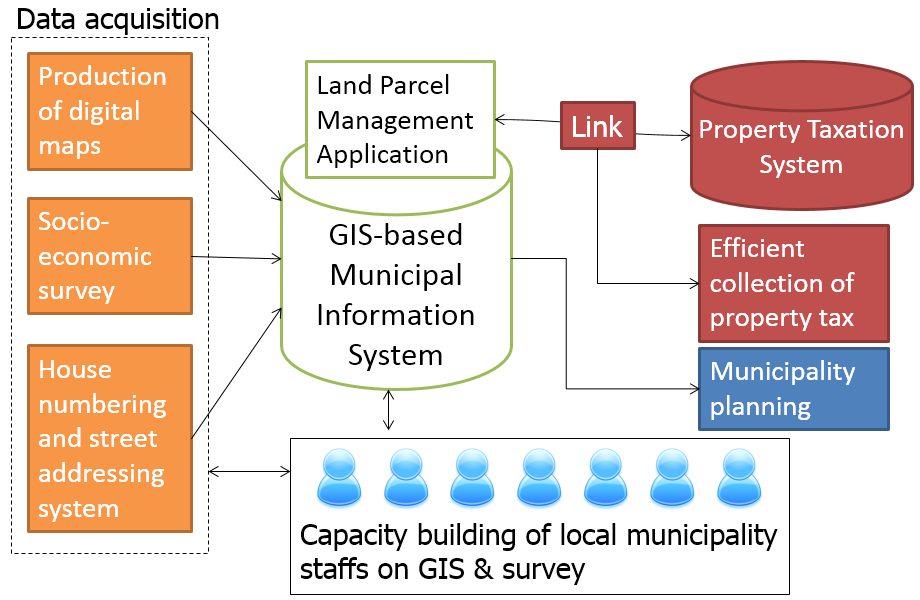
\includegraphics[width = 0.8\linewidth]{Figures/urban_nepal.png}
\end{center}
%\caption{urban_nepal}
\label{urban_nepal}
\end{figure}


\subsection{Improve the transportation sector}

\begin{itemize}

\item Significant improvement of management and operations by monitoring of both people/cargo movement and health of transportation infrastructure/vehicles.

\item Better safety by less incidents of transportation systems.

\item Reduction of disaster damages to transportation systems. Speedy evacuations of passengers and recovery of services

\item Data-driven, evidence-based planning of transportation infrastructure and healthy implementation of plans and operations.

\item Flexible adjustments of toll fees (road etc.) by location and time. Contribute to infrastructure development finance and better traffic controls.

\end{itemize}


\subsection{Improve the quality of life of people}

\begin{itemize}

\item Ensure people’s security by precisely delivered information about disaster and incidents.

\item Ensure epidemiological security by delivering precise risk information to people. 

\item Also provide health advices and information personalized by daily activities and exercises. These will improves efficiency of public health insurance.

\item Reduction of commuting time and traffic incidents by better traffic management. Safer and better quality of family life.

\item Better medical and health service efficiency by sharing location information of medical service resources, such as doctors, nurses, pharmacy, and instruments, in situations with limited resources.

\item More job opportunities and less unemployment rate by better job matching around home. And more safety by avoiding hazardous jobs by the better job opportunities.

\item Diverse education chances by various e-learning systems by ubiquitous network environments.

\item Promote community-based assistance through connections by location information and social media. This is very helpful in emergency responses.

\item Personal logs of activities and authenticated locations are utilized as proofs for individual authentication, anti-identity-spoofing and credit information of finances. It facilitates jobs of startups and small businesses via appropriate micro financing systems.

\end{itemize}


\subsection{Establish dynamic census}

\begin{itemize}

\item Nationally representative human mobility data with predicted demographic attributes

\item Advantages in data scarce environment

\item Safe-to-use because it is simulation data

\end{itemize}

\begin{figure}[H]
\begin{center}
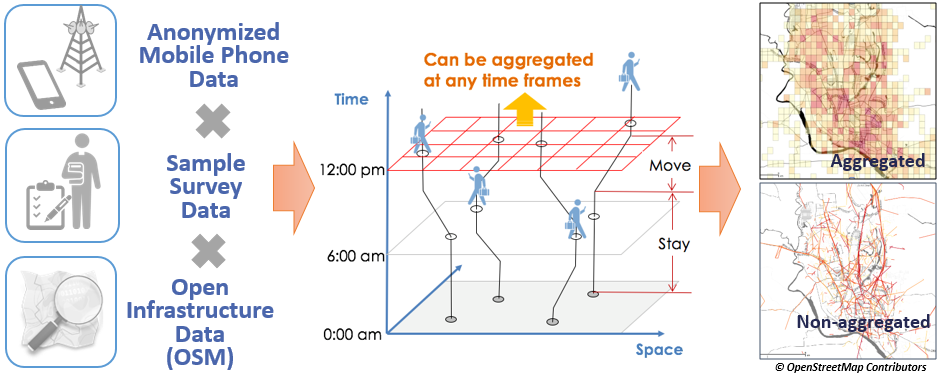
\includegraphics[width = 0.8\linewidth]{Figures/dynamic_census.png}
\end{center}
\caption{Schematic description of dynamic census}
\label{dynamic_census}
\end{figure}

{\flushleft \bfseries Example 1: Space-based Malaria Monitoring \& Control}

(Near) real-time mapping of malaria incidents and risks for decision support in malaria control by data collection, analysis, sharing, and visualization by combinations of space technologies and ground communications technologies. 

\begin{figure}[H]
\begin{center}
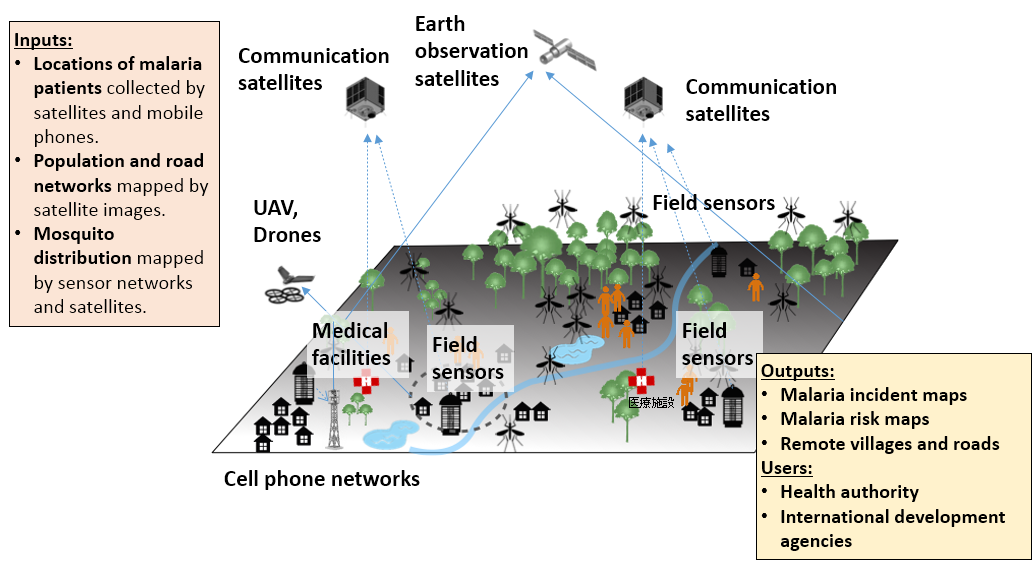
\includegraphics[width = 0.8\linewidth]{Figures/malaria.png}
\end{center}
\caption{(Near) real-time mapping of malaria incidents}
\label{malaria}
\end{figure}

{\flushleft \bfseries Example 2: People Monitoring for Ebola Control}

\begin{figure}[H]
\begin{center}
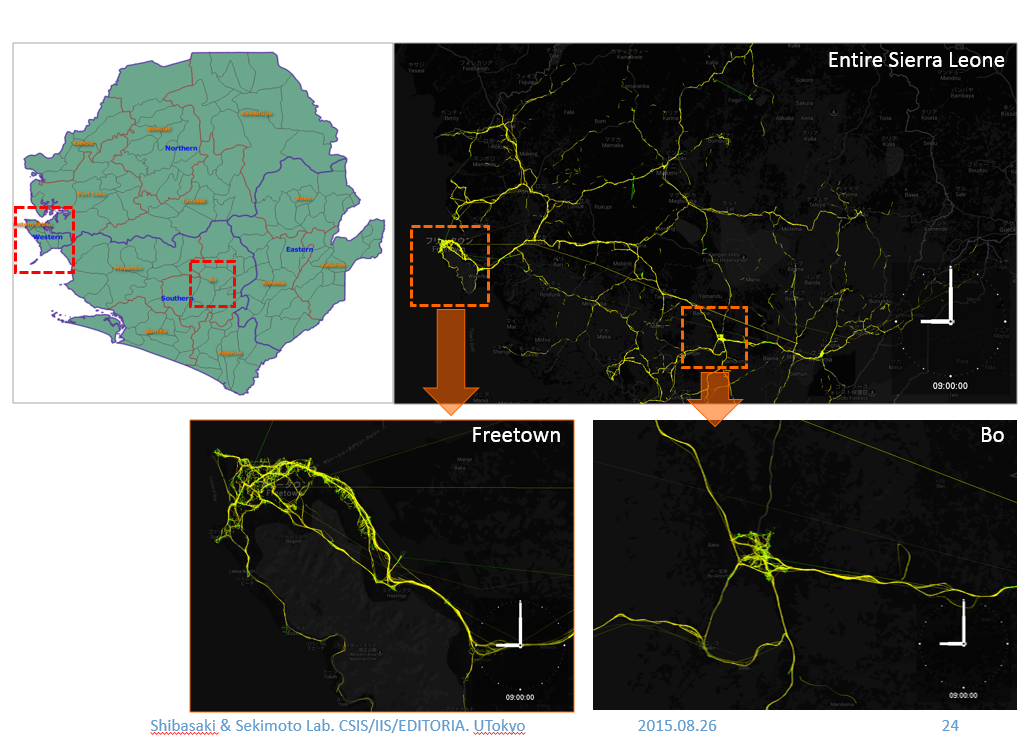
\includegraphics[width = 0.8\linewidth]{Figures/ebola.png}
\end{center}
\caption{People movement monitoring for Ebola control}
\label{ebola}
\end{figure}



\subsection{Enhance resilience}

\begin{itemize}

\item Reduce human damages by ensuring rapid information collection and delivery about disaster hazard and damages.

\item Ensuring goods delivery and debris removal by goods tracking and real-time recovery monitoring after disasters.

\item Higher accuracy of forecasts in ground/ocean weather information. Significant improvements are made using satellite earth observation. This provides industry and people  with lots of social benefits

\item By improving accuracy of monitoring and forecasting floods, slope failure, earthquake and volcanic eruptions, safety of people can be better secured.

\begin{figure}[H]
\begin{center}
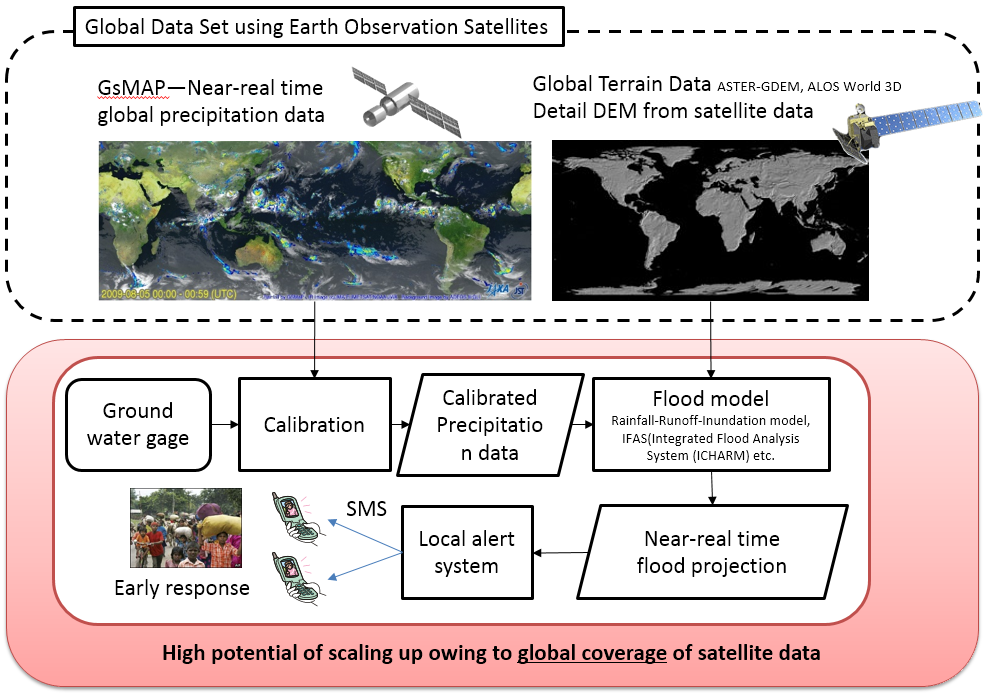
\includegraphics[width = 0.8\linewidth]{Figures/flood_alert.png}
\end{center}
\caption{Flood alert system with SGT}
\label{flood_alert}
\end{figure}

\item Disaster nursing supported with SGT.

\end{itemize}

\begin{figure}[H]
\begin{center}
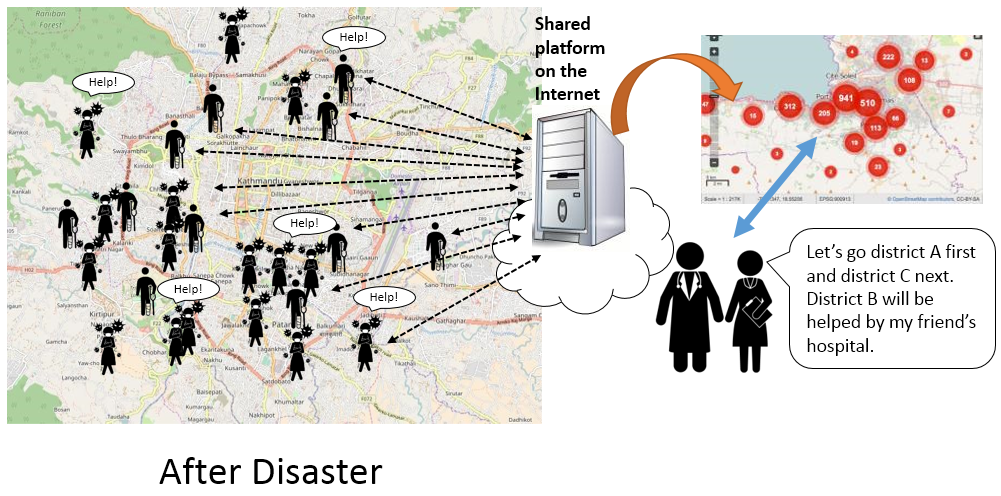
\includegraphics[width = 0.8\linewidth]{Figures/nursing.png}
\end{center}
\caption{Supporting disaster nursing with SGT}
\label{ebola}
\end{figure}

{\flushleft \bfseries Example: precipitation and flood monitoring in Bangladesh}

\begin{figure}[H]
\begin{center}
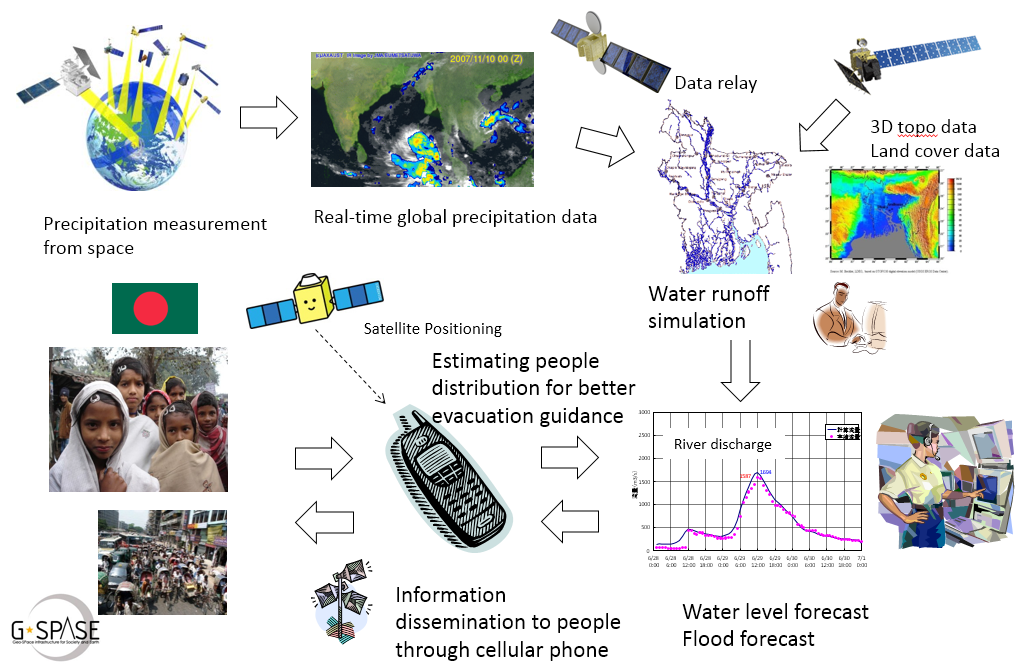
\includegraphics[width = 0.8\linewidth]{Figures/bangladesh.png}
\end{center}
\caption{Precipitation and flood monitoring in Bangladesh}
\label{bangladesh}
\end{figure}

\subsection{Improve logistics}

Track movement of things (cargos, freights) with authenticated position/time information, which enables:

\begin{itemize}

\item Certification of production place: more added-values by branding and safety, strengthening competitiveness and more activated industries and markets.

\item Less delivery loss and damages. Uber-like delivery service by average citizen. Smoother and cheaper logistic services. Strengthened logistic networks in remote areas, mountainous villages, and coastal areas.

\item More security and speed in custom clearance by certificates verified by authenticated mobility or location logs.

\item Securing collection, transport, and disposals of hazardous materials (e.g. industrial wastes) by movements monitoring. Contribute to environment conservation.

\item Reduction long-distance logistics cost by convoy transports of autonomous trucks on highways. ASEAN countries should have notable benefits owing to its dependency on road transports.

\item Much less operating cost and days by automation of container handling in harbors.

\end{itemize}

\subsection{Strengthen industrial activities}

\begin{itemize}

\item Agriculture

\begin{itemize}
\item Less damages by preparations to expected typhoons and hazardous weather, with adjusting timing of cropping, harvest, and shipping and so forth.
\item Optimized insurance cost by reducing agricultural risks and less compensation for agricultural damages from public sectors.
\end{itemize}

\begin{figure}[H]
\begin{center}
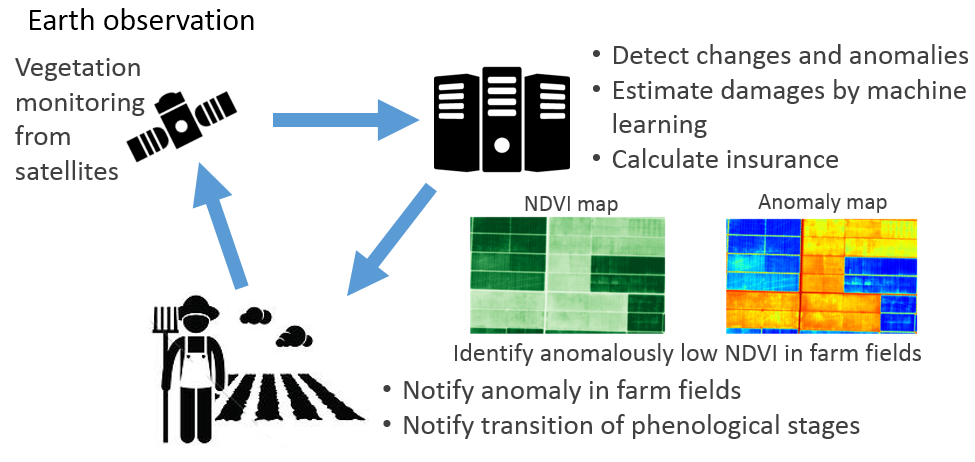
\includegraphics[width = 0.8\linewidth]{Figures/agri_anomaly.png}
\end{center}
\caption{SGT for agriculture}
\label{bangladesh}
\end{figure}

\item Fishery

\begin{itemize}
\item More efficient activities and operations of vessels and port facilities by forecasting harvestable areas and seasons. Better controlled market prices.
\item Less impact of oceanic hazards to fishery productions by meteorological forecasting. Better security by reduction of shipwreck. 
\item Better productivity and reduced disaster risks of aquaculture production by information of ocean condition and water quality (e.g. red tide).
\item Management of fishery resources, securing safe operations, and detection of suspicious vessels by tracking locations and operations of vessels with verified position authentication.
\end{itemize}

\begin{figure}[H]
\begin{center}
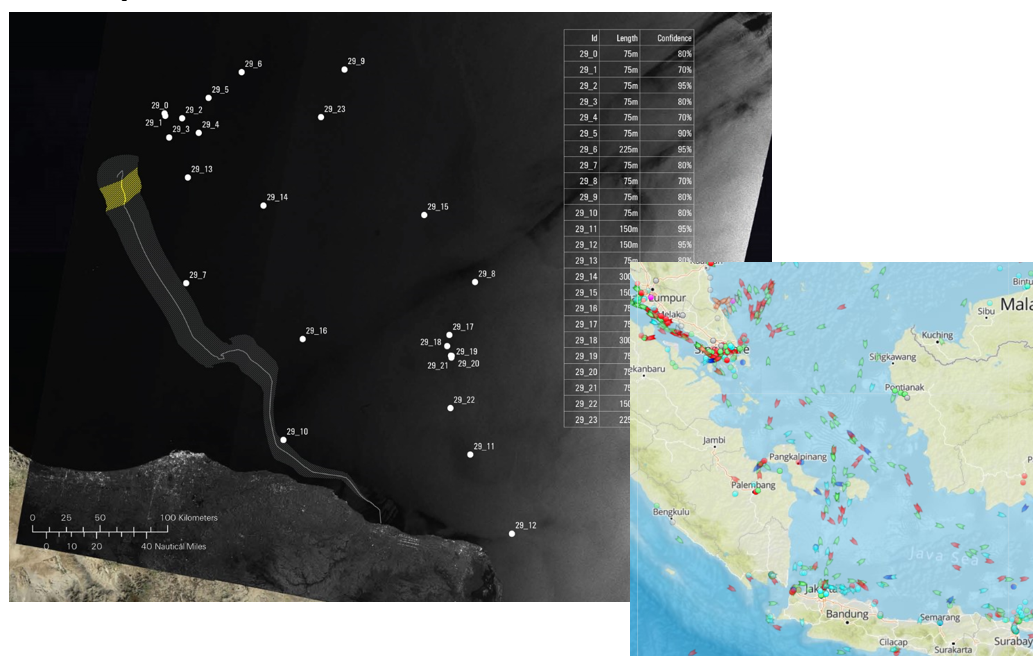
\includegraphics[width = 0.8\linewidth]{Figures/ship.png}
\end{center}
\caption{Unidentified ship detection by satellites and AIS/VMS}
\label{bangladesh}
\end{figure}

\item Forestry

\begin{itemize}
\item Ensure sustainable use of forest resources (planting, conservation, logging) by continuous monitoring of forest resources (biomass and tree types).
\item Better efficiency and effectiveness in logging, lumber, and transport by quantified planning of forestry operations. And less labor hazards.
\item Suppress damages of forest fire and illegal loggings.
\end{itemize}

\begin{figure}[H]
\begin{center}
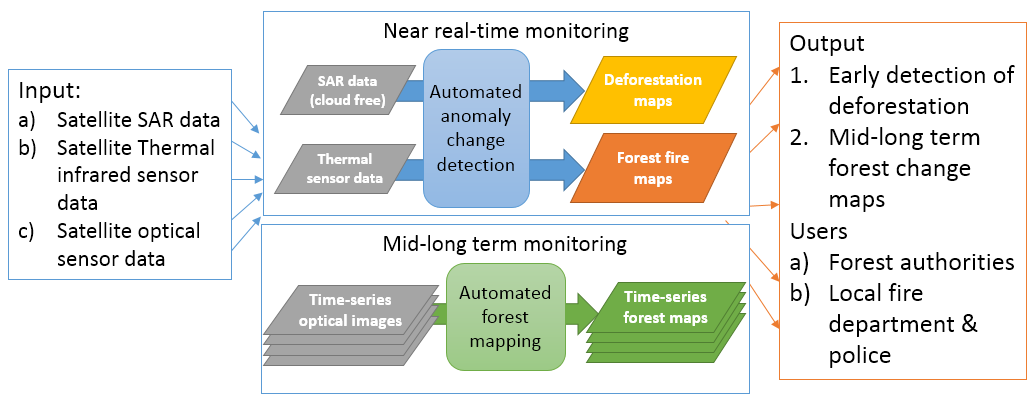
\includegraphics[width = 0.8\linewidth]{Figures/forest.png}
\end{center}
\caption{Forest monitoring with SGT}
\label{forest}
\end{figure}

\item Construction

\begin{itemize}
\item Risk reduction by effective designs and construction plans with accurately measured and shared data of terrain and geology.
\item Effective management of labors and staff safety with better efficiency of transports and stock usage by continuous and accurate monitoring of things and people’s position.
\item Quality assurance and improvement through detection and prevention of faults by accurate 3D measurement of construction progress.
\end{itemize}

\item Manufacturing

\begin{itemize}
\item Less logistics cost and uncertainty to deliver and procure products. Leading to cost reduction of manufacturing.
\end{itemize}

\item Service

\begin{itemize}
\item Less cost of service delivery by significant reduction of cost and uncertainty in logistics.
\item Realize possibilities of micro-consumer services, such as e-commerce and food delivery, by the low-cost and effective delivery services.
\item Better reliability of mobile payment using personal credit information based on locations and activities verified by positioning authentication. 
\item Scaling up of mobile micro consumer services by the more reliability of personal micro-payment systems.
\end{itemize}

\begin{figure}[H]
\begin{center}
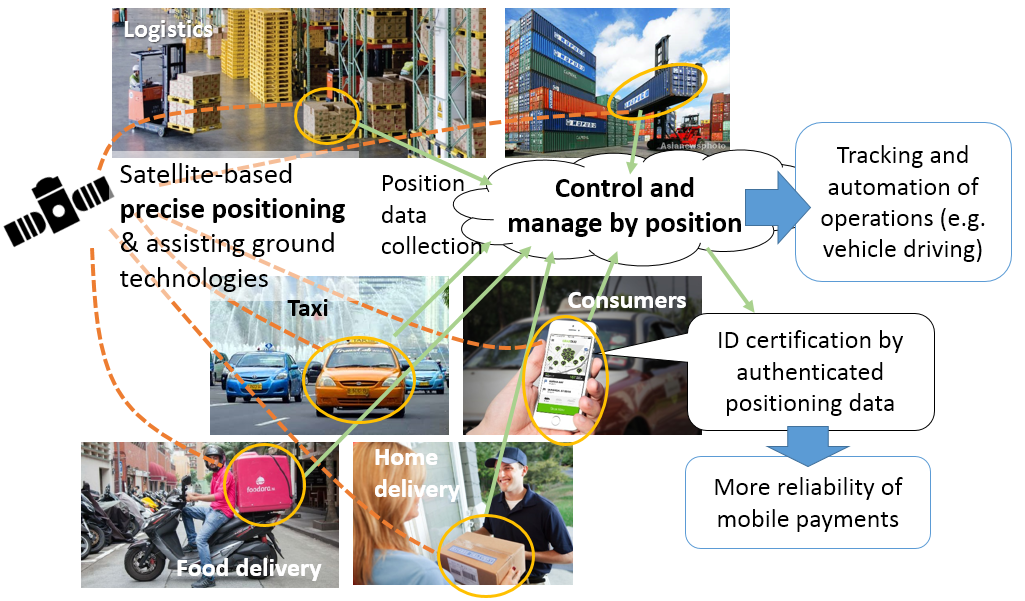
\includegraphics[width = 0.8\linewidth]{Figures/manufacturing_service.png}
\end{center}
\caption{SGT to support manufacturing and service sectors}
\label{manufacturing_service}
\end{figure}

\item Energy sector

\begin{itemize}
\item Energy demand and supply gaps visualized through satellite observations of city lights.
\end{itemize}

\begin{figure}[H]
\begin{center}
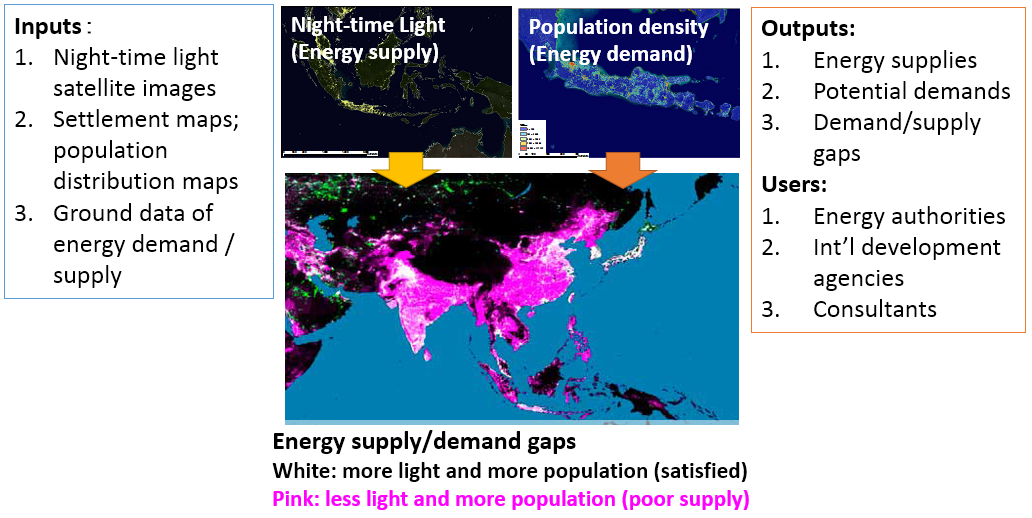
\includegraphics[width = 0.8\linewidth]{Figures/energy.png}
\end{center}
\caption{Estimating energy needs through night satellite observation}
\label{manufacturing_service}
\end{figure}

\end{itemize}

\subsection{Support environmental resources management}

\begin{itemize}

\item CO2 emission reduction by optimizing transport operations (taxi, commercial vehicles, and shipping vehicles) based on vehicle mobility data. This supports fund raising by environment finance scheme such as bilateral carbon offsets.

\item Effective conservation of ecosystem services by continuous monitoring of ecological status of forest, ocean, and marines.

\item Social bonds can be applied to better and sustain the services based on value evaluation of ecosystem services

\item Effective conservation and management of specific areas for species conservation and gene banks.

\end{itemize}

\begin{figure}[H]
\begin{center}
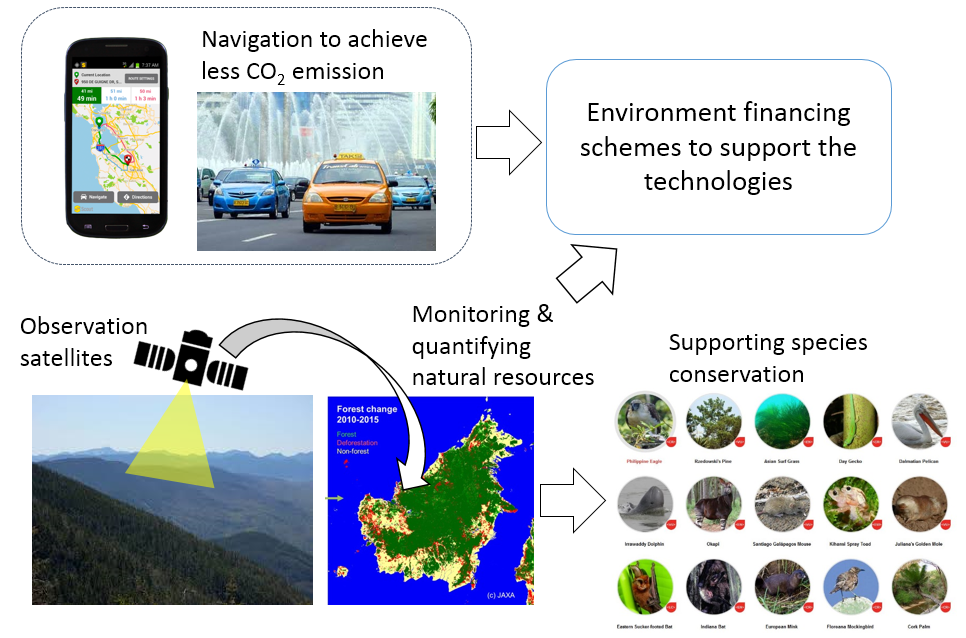
\includegraphics[width = 0.8\linewidth]{Figures/resource_manag.png}
\end{center}
\caption{SGT for environmental resources management}
\label{resource_manag}
\end{figure}

\subsection{Strengthen national land and sea management}

\begin{itemize}

\item Higher accuracy of forecasts in ground/ocean weather information using advanced satellite earth observation. This provides industry and people  with lots of social benefits.

\item Achieve marine safety and fishery resources conservation by strengthening detection and monitoring of unidentified ships.

\item Better safety/security of people by improving accuracy of monitoring and forecasting floods, slope failure, earthquake and volcanic eruptions.

\end{itemize}

\begin{figure}[H]
\begin{center}
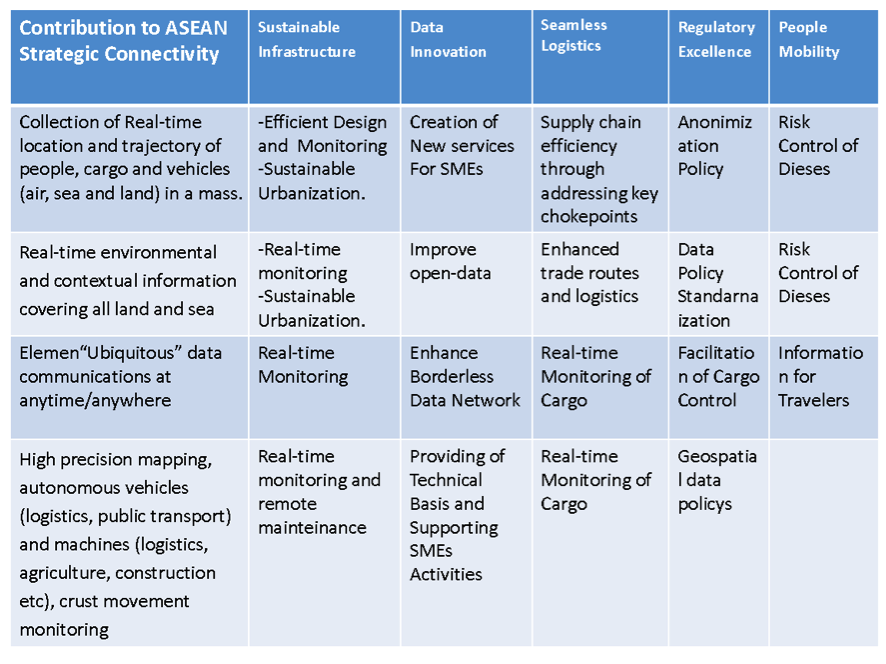
\includegraphics[width = 0.8\linewidth]{Figures/asean_connectivity.png}
\end{center}
\caption{Table asean connectivity}
\label{asean_connectivity}
\end{figure}



\section{Economic and industrial impacts -- Summary}

\begin{itemize}

\item Economic impacts of the improvement with SGT

\item Collecting examples...

	\begin{itemize}

	\item Traffic congestion

		\begin{itemize}

		\item Jakarta (Jakarta post 2015)
		
			\begin{itemize}
			\item 5 billion USD losses each year by traffic jam.
			\item 167 USD loss (person/year: 5\% of GDP per capita)
			\end{itemize}

		\item Nairobi, Kenya
		
			\begin{itemize}	
			\item 210 million USD loss each year 
			\item 60 USD loss (person/year: 5\% of GDP per capita).
			\end{itemize}

		\end{itemize}
	\end{itemize}
\end{itemize}


\chapter{Implications on ASEAN policies for better integration and connectivity}

\tab The previous chapters emphasized the benefits of Spatial and Geospatial Technology (SGT) for ASEAN, focusing on a wide range of issues such as logistics, disaster management or public health. This chapter adopts another perspective by looking at the implications on ASEAN policies of the enhancement of ASEAN connectivity through SGT.

\vspace{0.4 cm}

In particular, this chapter will be organized as follows:

\begin{enumerate}

\item What to realize with coordinated ASEAN policies?

\item ASEAN policies for Physical infrastructure

\item ASEAN policy directions for Sustainable value creation from data 

\end{enumerate}


\section{What to realize with coordinated ASEAN policies?}

\tab In order to benefit from the full potential of SGT, ASEAN countries will need to adopt coordinated policies aimed at establishing both a strong infrastructure supporting the use of SGT and a legal framework to organize SGT data utilization, as summarized below.

\begin{enumerate}

\item Physical infrastructure:

\begin{itemize}
\item Space systems: observation, positioning, and communication
\item Ground-based systems: base station networks, satellite communication points, and ground data networks
\end{itemize}

\item Data policies and associated public/industrial policies:

\begin{itemize}
\item Sustainable value creation from data by respecting rights and concerns of data producers and associated stakeholders.
\item Separation of data holdings/ownership and advanced usage by value creators/producers.
\item Sharing benefits among data producers and value creators.
\end{itemize}

\end{enumerate}

The next two sections further develops these necessary political goals.


\section{ASEAN Policies for Physical Infrastructure} \label{infrastructure}

\tab While it has immense potential benefits for the region, the utilization of SGT requires important initial investments for the establishment of highly-advanced  technological infrastructures, both in outer space and at ground level.


\subsection{Space systems: observation, positioning, and communication}

\subsubsection{Earth observation}

\tab Concerning the use of earth observation technologies, we recommend different approaches depending on the kind of application requested.

\begin{enumerate}

\item In the case of \textbf{global earth observation}, the cost of establishing a large constellation of expensive satellites would be unbearable for ASEAN countries, even if united behind this goal. Therefore, it would be beneficial for ASEAN to \textbf{join global earth observation open data clubs} such as the \textit{Group on Earth Observations}.

\item In the case of \textbf{local observation}, ASEAN countries could develop indigenous capabilities through the establishment of regional policies balancing between competition and collaboration. We recommend two approaches, which can be followed in parallel:

	\begin{enumerate}
	\item \textbf{ASEAN satellites}. Joint development/operation of ASEAN satellites by member countries under the banner of ASEAN. We could even imagine the establishment of an ASEAN satellite constellation.
	\item \textbf{National satellites}. Individual development of satellites by member countries, eventually participating in an ASEAN constellation.
	\end{enumerate}

\end{enumerate}

Two supplementary comments can be made regarding the development of local observation capabilities:

\begin{enumerate}

\item A strong focus has been made on the \textbf{importance of the establishment of an ASEAN constellation}. Facing the same challenges on a relatively similar environment and having a solution --- SGT --- transcending by definition national boundaries, it would be highly inefficient for ASEAN member countries to develop in parallel similar technologies without collaborating. Moreover, beyond simple data sharing, the coordinated operation of various ASEAN satellites would improve the efficiency of SGT by allowing an increase in covered area and/or of revisit frequency of the satellites.

\item Beyond regional utilization, the data produced by ASEAN satellites could then be shared in a previously mentioned global earth observation open data club.

\end{enumerate}

\subsubsection{Satellite positioning systems}

The ongoing GNSS operations are operated by independent bodies though the operations have potentials to collaborate for better services supported by high-precision and real-time positioning technologies. It is useful to design such collaborative systems by i) space segment, ii) control segment, and iii) user segment.

\subsubsection*{Space segment}

The space segment covers designs operations of satellites, such as structuring constellation satellites. As well as the earth observation, regional cooperation in satellite operations shall be beneficial to participating countries through the mechanism of infrastructure sharing. Currently, Asia and Pacific region is the most intensive GNSS coverage than other regions owing to GPS, GLONASS, Galileo, Compass, IRNSS, and QZSS. Especially, QZSS is a GNSS constellation dedicating East Asia, Southeast Asia, and Oceania by its orbits focusing the areas. International cooperation of QZSS applications could be expected to be a model promoting regional positioning satellite systems.

\subsubsection*{Control segment}

The control segments includes infrastructure to observe the movement of the satellites and computing orbit data (ephemeris), and to monitor the satellite clock and computing their correction parameters, which are basis of high-precision positioning techniques, such as RTK and Precise Point Positioning (PPPo). The MADOCA high-precision positioning is realized by data management and processing of signals from space and delivery of processed data to user segment. Continuous Operational Reference Station (CORS) can be included in the control segment because of its positions as a ground infrastructure though it is somewhat likely in user segment because it comprises user segment technologies.

While PPPo does not need cooperation among operational bodies because of its independence from ground reference points, RTK needs certain cooperation among operational bodies as positioning accuracy of RTK is affected by proximity to reference stations. Integration of the reference stations infrastructure, especially CORS network, should be beneficial for GNSS user segments to provide high-precision positioning data to applications. There are two considerable issue in regional integration of CORS infrastructure.

\textbf{Intra-country cooperation} - It sometimes challenging to integrate CORS networks even within a country because CORS operation bodies spread from public sectors to private sectors, in which data policy varies in wide ranges. Approaching as an international cooperation requires dialogues with each operating body unless single-window mechanisms are established. For example of Thailand, public CORS operating bodies are Royal Thai Survey Department, 
Hydro and Agro Informatics Institute, Department of Land, GISTDA, and Department of Public Works and Town & Country Planning. An international mission had to construct agreements with each agencies to use their CORS infrastructure. Recently, the government of Thailand concluded a single-window policy of international cooperation on use of CORS network in Thailand, with which the Royal Thai Survey Department shall take responsibility to coordinate international cooperation with the operating agencies. The practice of Thailand will be a good model to recommend the ASEAN states to develop a policy for better integration of CORS networks within their countries.

\textbf{Inter-country cooperation} - The CORS networks sometimes contribute to high-precision positioning beyond borders, especially for border areas with little density of reference stations. Data transfer beyond boarders are another challenging issue because the CORS data is a military-sensitive information. Developing agreements shall be initiated by specific applications with tangible benefits competitive to political sensitivity. At a stage with a certain number of agreements concluded, ASEAN may recommend the states to develop a multi-lateral agreement on use of CORS networks over the ASEAN states.

\subsubsection*{User segment}

In the past, RTK-GPS instruments had been mainly for professional surveys and costed tens of thousand dollars. Instead, only hand-held GPS devices were affordable to consumers. However, in the last few years, low-cost RTK devices are available at costs of hundreds dollars. In addition, more smart phone penetrations reaching high-precision positioning service owing to the hybrid positioning using GNSS and celltower-based positioning. Although this consumer market trends and growths are rather independent from the governments' policies, the ASEAN policy shall include these status and projections.

\subsubsection{Satellite communications}

While satellite communications are regarded as a key technology for IoT applications, operation costs are considerably high for ASEAN states. Store and forward is a technique to reduce costs of satellite communications, in which a satellite receives data from a ground transmitter when the satellite visit over the transmitter, store the data on the satellite, adn transmit the data to a ground receiver when the satellite visit over the ground receiver. Store and forward reduces communication costs at an expense of update frequency. The store and forward is expected to apply to sensor networks in areas without land-line internet connections, such as remote areas and oceans. The technology could support ASEAN states in continuous monitoring of environment and disasters in a sustainable way by the low-cost advantage.

\subsection{Ground-based systems}

\tab The second type of infrastructures which will need to be promoted through ASEAN policies are ground systems. In particular, we recommend the development of three different categories of ground systems.

\begin{enumerate}

\item \textbf{Base station networks}. National development of base stations --- necessary for the downlink of data produced by observation satellites or gathered by communication satellites from ground measurement stations --- to form international networks. By having a large network of interconnected base stations, real-time data exchange will be available for ASEAN countries, however conditioned to the interoperability of base stations.

\item \textbf{Satellite communication points}. Individual development with interoperability.

\item \textbf{Ground data networks}. Individual development of ground measurements stations, emitting \textit{in-situ} data towards ASEAN communication satellites. Therefore, the adoption of common data standards will be necessary for the functioning of the full system.

\end{enumerate}

The keyword here in \textbf{interoperability}. Contrary to satellites which are moving in outer space, a neutral area for international law, ground stations will be placed on the exclusive territories of ASEAN member states. Therefore, to use the potential of such a wide network, it is necessary to ensure the \textbf{compatibility} between all infrastructures and facilitate the \textbf{adoption of common standards} throughout ASEAN.


\section{ASEAN policy directions for Sustainable value creation from data} \label{data_util}

\tab This section aims at answering the following question: how to sustain value creation from data, while respecting the rights and concerns of data producers and associated stakeholders?

\vspace{0.4 cm}

To answer this question, we recommend to follow specific policy directions, consisting in the adoption of coordinated data policy for advanced usage. In particular, focus should be placed on:

\begin{enumerate}

\item \textbf{Separating data holdings/ownership and advanced data usage and integration by value creators}, as well as \textbf{respecting rights and concerns of data producers/stakeholders}. In other words, ensuring a smoother flow of data and a clearer responsibility of data usage.

\item \textbf{Sharing the benefits of value creation from data} among data producers and value creators.

\item \textbf{Monitoring and assessing risks and benefits of data usage} and data market competition/concentration in a coherent manner.

\item \textbf{Accelerating human resource development} of value creation.

\end{enumerate}


\begin{figure}[H]
\begin{center}
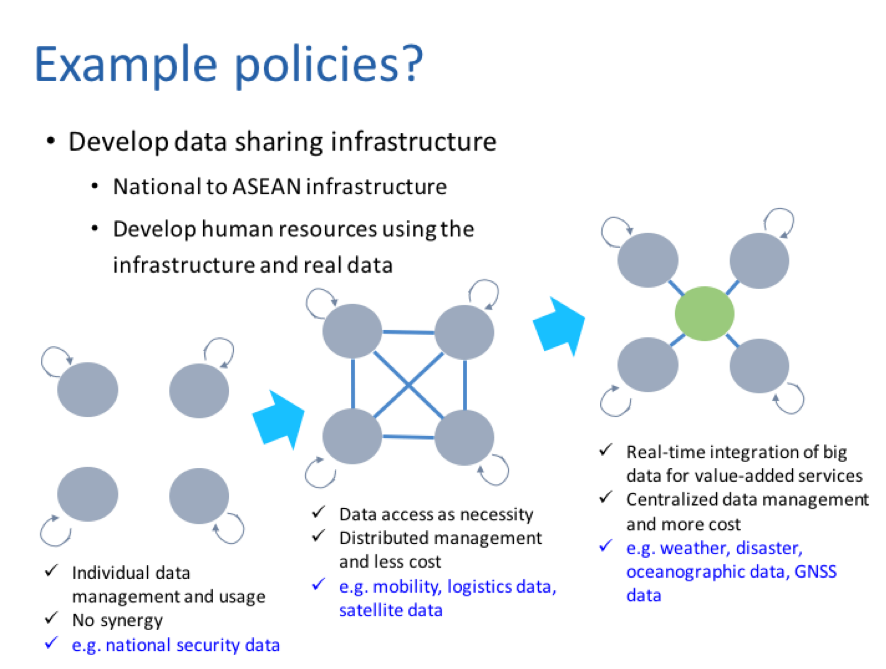
\includegraphics[width = 0.8\linewidth]{Figures/example_policies.png}
\end{center}
\caption{Example policies}
\label{example_policies}
\end{figure}




\chapter{Roadmap for connectivity enhancement and Flagship Projects}

\tab Based on all the issues presented and the solutions proposed in the previous chapters, this chapter summarizes the key development areas for the enhancement of ASEAN connectivity and resilience. ASEAN countries being divided in two categories, insular and continental, it is necessary to take into account their relatives specificities.

Therefore, this chapter differentiates between land connectivity and ocean connectivity, and proposes recommendations aiming at their enhancement. For each of them, after stating precise targets, we recommend specific actions which should be carried out to achieve those targets.

\section{Better Land Connectivity} \label{land}

\tab More than half of ASEAN countries --- in alphabetical order, Cambodia, Lao P.D.R., Malaysia (partially), Myanmar, Singapore, Thailand, and Vietnam --- are continental. Therefore, enhancing land connectivity is a great priority for ASEAN.

\begin{figure}[H]
\begin{center}
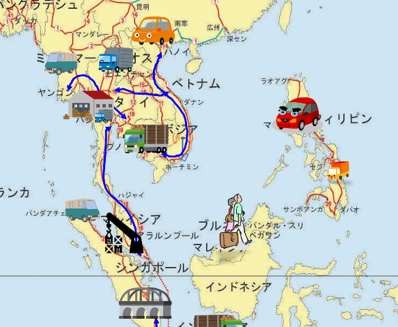
\includegraphics[width = 0.8\linewidth]{Figures/land_connect.png}
\end{center}
\caption{Improved land connectivity with SGT}
\label{land_connect}
\end{figure}

\subsection{Targets}

\begin{enumerate}

\item Smoother and safer transport, logistics, and people flow 

\begin{itemize}
\item Drastic cost reduction and accident reduction for mobility
\end{itemize}

\item Better and secure management of transportation (e.g. road pricing, cargo management, people mobility management)

\begin{itemize}
\item Better security and management, reduction of GHGs
\end{itemize}

\item Accelerating implementation of  autonomous vehicles, automation in transport, logistics, construction, agriculture/forestry etc.

\begin{itemize}
\item Advanced/leading technologies and implementation
\end{itemize}

\item Providing advanced positioning services for safer mobility

\begin{itemize}
\item World-first services for safer and securer mobility
\end{itemize}

\end{enumerate}

\subsection{Actions}

\begin{enumerate}

\item Develop incubation centers of advanced positioning services and applications

\begin{enumerate}
\item High precision, authentication (anti-spoofing)
\item Support of industrial development and business creation.
\item Model case; GNSS incubation center (GISTDA, Thailand)
\end{enumerate}

\item Establish connected networks of GNSS base stations

\begin{enumerate}
\item Common location basis of ASEAN for better consistency and accuracy
\item High-precision mapping, autonomous vehicle (logistics, public transport) and machines (logistics, agriculture, construction etc.), crust monitoring
\item Enhancing NSDI (National Spatial Data Infrastructure) to better geospatial data dissemination and integration
\end{enumerate}

\item Provide world-first advanced positioning services

\begin{enumerate}
\item Free high precision, authentication service with QZSS
\item Accelerate social implementation: Road pricing, Illegal vehicle detection, Secure logistics
\end{enumerate}

\item Develop data sharing infrastructure and human resource development facility

\begin{enumerate}
\item Logistics, transportation, people flow, autonomous vehicle etc.
\item Incubation of data experts serving better data usage and management
\end{enumerate}

\end{enumerate}


\section{Better Sea Connectivity} \label{sea}

\tab Four ASEAN countries are either fully or partially insular --- in alphabetical order, Brunei Darussalam, Indonesia, Malaysia (partially), and the Philippines --- and include some of the leading Asian economies such as Indonesia. Moreover, with the exception of Lao P.D.R., all ASEAN countries have access to the sea, prompting the improvement of sea connectivity.

\begin{figure}[H]
\begin{center}
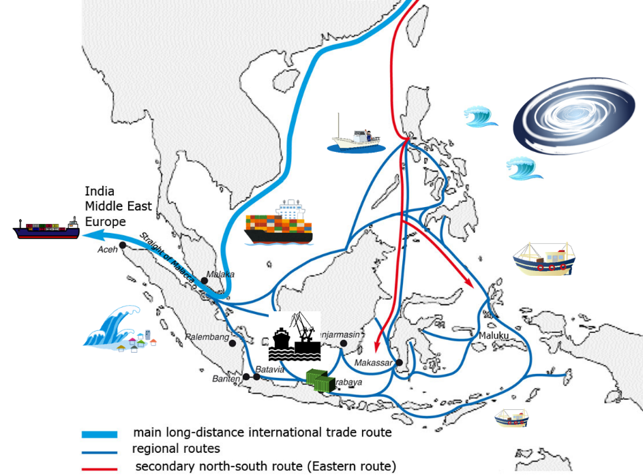
\includegraphics[width = 0.8\linewidth]{Figures/sea_connect.png}
\end{center}
\caption{Improved sea connectivity with SGT}
\label{sea_connect}
\end{figure}

\subsection{Targets}

\begin{enumerate}

\item Smoother and safer transport and logistics in the seas.

\item Reduction of cost/time and marine incidents.

\item Safer and securer industrial activities in the seas.

\item Accident reduction and better control of sea activities.

\item Sustainable management and development of natural resources.

\item Control of natural resource development and conservation of ecosystems.

\end{enumerate}

\subsection{Actions}

\begin{enumerate}

\item Develop marine weather forecast and application center

	\begin{enumerate}
	\item More accurate and integrated marine weather monitoring and forecast

		\begin{enumerate}
		\item Numerical models, data assimilation, satellite data like Himawari
		\end{enumerate}
	
	\item Provide marine data for marine industrial activities such as fishery and aquaculture
	\item Incubate advanced applications for fishery, aquaculture, and environmental management
	\item Model case: IMRO (Indonesia)
	\end{enumerate}

\item Expand world-first advanced positioning services

	\begin{enumerate}
	\item Free and precise, authentication service with QZSS in the seas and ocean
	\item Accelerate social implementation: monitoring and control of fishery, detecting unidentified ships, secure marine logistics, automation of cargo handling etc.
	\end{enumerate}

\item Develop data sharing infrastructure and human resource development facility

	\begin{enumerate}
	\item Marine and land weather, marine logistics, transportation, etc.
	\item Integration of space data and in-situ data
	\item Incubation of data experts serving better data usage and management
	\end{enumerate}

\end{enumerate}


\section{Flagship projects for the development of data sharing infrastructure and related human resources} \label{flagship}

\tab In order to demonstrate the efficiency of SGT in the enhancement of ASEAN connectivity, we present potential flagship projects as well as implementing agencies.

\vspace{0.4 cm}

In particular, beyond the development of data sharing space infrastructure (satellite and ground systems), these projects aim at:

\begin{enumerate}
\item Promoting human resource development for advanced data analysis and usage, including Artificial Intelligence and Internet of Things (IoT) technologies.
\item Demonstrating best practices of data sharing and integration
\end{enumerate}

Concretely, the proposed flagship projects focus on:

\begin{enumerate}

\item Land applications focusing on positioning services, implemented by the GNSS Innovation Center of the Geo-Informatics and Space Technology Development Agency (GISTDA) of Thailand.

\item Marine applications driven by the Institute for Marine Research and Observation (IMRO) of Indonesia.

\item Disaster response and risk management, supervised by the AHA Centre, based in Jakarta, Indonesia.

\item National Space Data Infrastructure and geospatial application centers in each member country.

\end{enumerate}



\addcontentsline{toc}{chapter}{Conclusion}
\chapter*{Conclusion}

\tab The rise of Space and Geospatial Technology had a deep impact on all layers of society. By combining a highly technological space infrastructure (earth observation, positioning and communication) with new technologies for data utilization (AI, IoT, etc.), the contribution of SGT for the economy is already visible but should be further promoted (\ref{wi_sgt}). 

\vspace{0.4 cm}

More specifically, SGT could participate in the realization of the 2025 ASEAN vision of increased resiliency and connectivity. In 2016, the \textit{Master Plan on ASEAN Connectivity 2025} itself reaffirmed the importance of space technologies and data sharing for regional economic development (\ref{enhanced}). As explained previously in this report, SGT can play a prominent role in the global optimization of ASEAN production system (\ref{optimization}) and the transformation of the economy with the third unbundling (\ref{unbundling_p}). SGT will also help ASEAN to develop an ambitious vision towards the status of Data-Driven Innovation Economy 2.0.

\vspace{0.4 cm}

It is therefore primordial for ASEAN member countries to develop a common vision and common policies towards the establishment of an efficient physical infrastructure for data collection in ASEAN (\ref{infrastructure}). It will also be necessary to create a regional data policy for data utilization and data format standardization (\ref{data_util}).

\vspace{0.4 cm}

Finally, several ambitious flagship projects should be implemented for the increase of both land (\ref{land}) and sea connectivity (\ref{sea}) and for the continuous development of human resources with adaptive systems (\ref{flagship}). It will support the promotion, maintaining and enhancement of the feeling of "We" and deepening the sense of ASEAN identity.






\appendix
\chapter{Summary of the workshops}


\section{ERIA Forum during APRSAF -- Manila, November 2016}

\subsection{Agenda}

{\flushleft

\textbf{Time}: 15:00-18:00, 18 November 2016

\vspace{0.4 cm}

\textbf{Venue}: Leyte Room, Sofitel Philippine Plaza Manila

\vspace{0.4 cm}

\textbf{Participants}:

\begin{itemize}
\item ASEAN -- 10 people from Indonesia, Malaysia, Philippines, Thailand, Vietnam
\item Japan -- 20 people incl. DDG of Cabinet Office, NIED, RESTEC, JSS, JSF, universities (UT, KIT, Yamaguchi), PASCO and AXELSPACE
\end{itemize}

\vspace{0.4 cm}

\textbf{Agenda}:

\begin{enumerate}

\item Opening and Overview of ERIA project

	\begin{enumerate}
	\item Opening Remarks (3M)
	
	\textit{Cabinet Office, GoJ}
	\item ASEAN Roadmap for Regional DRM Cooperation: Objective of ERIA Forum and Discussion Points (10M)
	
	\textit{Hiroyuki Miyazaki, The University of Tokyo}
	\item Perspectives of ERIA and ADB's Strategies in Asian Cooperation (5M)
	
	\textit{Quentin Verspieren, The University of Tokyo}
	\end{enumerate}

\item Toward Enhancement of Resilience by Using Space Technology

	\begin{enumerate}

	\item Geospatial Information (Positioning Information, Big Data, GNSS Reference Station, etc.)
	
		\begin{enumerate}
		\item Deployment of GNSS Reference Station (8M)
		
		\textit{Tadashi Sasagawa, PASCO}
		\item Expectation for High Precise Positioning Service (7M)
		
		\textit{Peraya Tantianuparp, Hydro and Agro Informatics Institute (HAII)}
		\item Case Studies of DRM services using Geospatial Information/Positioning Technologies (15M)
		
		\textit{Masahiko Nagai, Yamaguchi University}
		\item Remote Sensing and Big Data Analysis for DRM (5M)
		
		\textit{Hiroyuki Miyazaki, The University of Tokyo}
		\end{enumerate} 

	\item Utilization of Satellite Data
		
		\begin{enumerate}
		\item SDGs and Climate Change Adaptation—A Pilot Project on Index-based Insurance for Agriculture (10M)
		
		\textit{Kazushi Motomura, RESTEC}
		\item Ocean Monitoring (e.g. Oil Spill, Coastal Zone Monitoring): Utilization of Satellite Data (ASTER, Hyperspectral Data, etc.) (15M)
		
		\textit{I Nyoman Radiarta, Institute for Marine Research and Observation (IMRO)}
		
		\textit{Osamu Kashimura, Japan Space Systems}
		\item Store and Forward Communication (5M)
		
		\textit{Toshihiro Obata, The University of Tokyo}
		\item Nano-satellite (10M)
		
		\textit{George Maeda, Kyushu Institute of Technology}
		\item Small Satellite Constellation (7M)
		
		\textit{Yuya Nakamura, AXELSPACE}
		\item Introduction of DIAS and Himawari Data (10M)
		
		\textit{Hiroyuki Miyazaki, The University of Tokyo (on behalf of Prof. Ryosuke Shibasaki)}
		\end{enumerate}

	\end{enumerate}
	
\item Workshop (60M)
	
	\begin{itemize}
	\item Brainstorming of Core Services and Symbolic Projects for Future Cooperation
	\item Needs from ASEAN Countries
	\end{itemize} 

\item Closing Remarks
	
\textit{Cabinet Office, GoJ}

\end{enumerate}
}

\subsection{Details on the workshop}

\tab The objective of this workshop was to identify core-examples of the utilization of SGT in ASEAN, through intense discussions among participating specialists. Then a specific focus was given on the potential for ASEAN-wide scale up of the examples.

\vspace{0.4 cm}

The guest specialists were divided into four groups moderated by organizers associating a specific issue (disaster risk management or ocean-related applications) with a specific technology (Earth observation or position systems):

\begin{enumerate}

\item Disaster risk management \& Earth Observation

\item Disaster risk management \& Positioning

\item Ocean \& Earth Observation

\item Ocean \& Positioning

\end{enumerate}



\section{ERIA Wrap-up Forum -- Jakarta, July 2017} \label{ws_jakarta}


\subsection{Agenda}

{\flushleft

\textbf{Time}: 12:00-15:30, 6 July 2017 (11:00-12:00 Registration and Lunch)

\vspace{0.4 cm}

\textbf{Venue}: Headquarters of ERIA

\vspace{0.4 cm}

\textbf{Address}: Sentral Senayan II, 6th floor Jalan Asia Afrika No.8, Gelora Bung Karno, Senayan, Jakarta Pusat 10270, Indonesia

\vspace{0.4 cm}

\textbf{Participants}:

\begin{itemize}
\item ASEAN -- 10 people from Indonesia, Malaysia, Philippines, Thailand, Vietnam
\item Japan -- 20 people incl. DDG of Cabinet Office, NIED, RESTEC, JSS, JSF, universities (UT, KIT, Yamaguchi), PASCO and AXELSPACE
\end{itemize}

\vspace{0.4 cm}

\textbf{Agenda}:

\begin{enumerate}

\item Opening and Overview of ERIA project

	\begin{enumerate}
	\item Opening Remarks (3M)
	
	\textit{Mr. Takashi Ikeda, Cabinet Office, GoJ}
	\item ASEAN Roadmap for Regional DRM Cooperation: Objective of ERIA Forum and Discussion Points (20M and 10M Q\&A)
	
	\textit{Prof. Ryosuke Shibasaki, The University of Tokyo}
	
	\textit{Prof. Takayoshi Fukuyo, The University of Tokyo}
	
	\textit{Prof. Hiroyuki Miyazaki, The University of Tokyo}
	
	\textit{Mr. Quentin Verspieren, The University of Tokyo}
	\item Perspectives of ERIA and ADB's Strategies in Asian Cooperation (5M)
	
	\textit{Quentin Verspieren, The University of Tokyo}
	\end{enumerate}

\item Possible Core Examples Toward Envisaged Sustainable Scheme of Geospatial/ Space‐based Service in ASEAN Region

	\begin{enumerate}
	\item Indonesia
		
	\textit{Dr. I Nyoman Radiarta, IMRO (10M and 3M Q\&A)}
	
	\textit{Mr. M. Rokhis Khomarudin, Remote Sensing Application Center, LAPAN}
	\item Lao PDR (12M and 3M Q\&A)
		
	\textit{Ms. Xaysomphone Souvannavong, Department of Disaster Management and Climate Change, Ministry of Natural Resource and Environment}
	\item Malaysia (12M and 3M Q\&A)
		
	\textit{Dr. Abdul Rashid Mohamed Shariff, Universiti Putra Malaysia (UPM)}
	\item Myanmar (12M and 3M Q\&A)
		
	\textit{Ms. Daw Thiri Maung, Ministry of Social Welfare, Relief and Resettlement}
	\item Philippines (12M and 3M Q\&A)
		
	\textit{Mr. Adrian Josele Quional/ Mr. Alvin Familara, National SPACE Development Program}
	\item Thailand (12M and 3M Q\&A)
		
	\textit{Mr.Jakrapong Tawala, GISTDA}
	\item Vietnam (12M and 3M Q\&A)
		
	\textit{Mr. Vu Anh Tuan, Vietnam National Satellite Center (VNSC)/Vietnam Academy of Science and Technology (VAST)}
	\end{enumerate} 

\item Discussions (60M)
	
	\begin{itemize}
	\item Developing sustainable collaboration model for implementing integrated space‐ based/geospatial socio-economic platform to strengthen the resilience in ASEAN community
	\item Next Step of the Project
	\end{itemize} 

\item Closing Remarks
	
\textit{Cabinet Office, GoJ}

\end{enumerate}
}

\subsection{Details on the workshop}

The discussion part witnessed very interesting debates and comments from all present members, which spirit can be found in the 'abstract' they send us after the workshop. These abstracts can be found, unedited, in appendix \ref{abstracts}.









\chapter{Summary of field visits and interviews}

\tab This appendix presents the list of field visits and interviews carried out for this project. They aimed at gathering the concerns, needs and experience from regional practitioners, both from ASEAN governments and regional institutions.

\vspace{0.4 cm}

All visits and interviews were carried out by Prof. Hiroyuki Miyazaki and Mr. Quentin Verspieren.

\section{Nay Pyi Taw, Myanmar -- October 25, 2016}

\begin{table}[H]
   %\caption{ }
   \centering
   \begin{tabular}{| c | p{12 cm} |}
   \hline
    Place & Emergency Operations Center (EOC), Relief and Resettlement Department (RRD), Ministry of Social Welfare, Relief and Resettlement (MSWRR), Nay Pyi Taw, Myanmar \\ \hline
    Date (Time) & October 25, 2016 (10:00--12:30) \\ \hline
    Counterpart & Ms Thiri MAUNG, Deputy Director of the EOC \\ \hline   
   \end{tabular}
\end{table}

Main elements of the discussion:

\begin{itemize}

\item Role and responsibilities of the EOC.

\item Future version of the \textit{Myanmar Action Plan for Disaster Risk Reduction}.

\item Importance of improving emergency information dissemination.

\item Consequences of the Nargis Cyclone.

\item Overview of Myanmar's international collaborations for disaster reduction.

\item Structural problems of disaster management in Myanmar

\end{itemize}



\section{Vientiane, Lao P.D.R. -- January 30, 2017}


\subsection{Disaster preparedness and response division, MONRE}

\begin{table}[H]
   %\caption{ }
   \centering
   \begin{tabular}{| c | p{12 cm} |}
   \hline
    Place & Disaster Preparedness and Response Division (DPRD), Department of Disaster Management and Climate Change (DDMCC), Ministry of Natural Resources and Environment (MONRE), Vientiane, Lao P.D.R. \\ \hline
    Date (Time) & January 30, 2017 (9:45--11:25) \\ \hline
    Counterparts & \begin{itemize} \item Ms Sonephet PHOSALATH, director of the DPRD \item Mr. Xailee XAYAXANG, technical officer at the DPRD  \end{itemize} \\ \hline   
   \end{tabular}
\end{table}

Main elements of the discussion:

\begin{itemize}

\item Organization of disaster management in Lao P.D.R.

\item Governmental efforts and inter-ministerial collaborations for disaster management.

\item Access to geospatial data from international partners (Japan and Sentinel Asia in particular).

\end{itemize}


\subsection{Natural Resources and Environment Institute, MONRE}

\begin{table}[H]
   %\caption{ }
   \centering
   \begin{tabular}{| c | p{12 cm} |}
   \hline
    Place & Office of the Deputy Director General, Natural Resources and Environment Institute (NREI), Ministry of Natural Resources and Environment (MONRE), Vientiane, Lao P.D.R. \\ \hline
    Date (Time) & January 30, 2017 (11:25--12:30) \\ \hline
    Counterparts & \begin{itemize} \item Mr. Phetsamone DALALOM, Deputy Director General of the NREI \item Ms Sonephet PHOSALATH, director of the DPRD \item Mr. Xailee XAYAXANG, technical officer at the DPRD \item 3 technical officers of the Remote Sensing Center (RSC), NREI \end{itemize} \\ \hline   
   \end{tabular}
\end{table}

Main elements of the discussion:

\begin{itemize}

\item Presentation of the Remote Sensing Center's activities and current capabilities.

\item Interactions between the RSC and Sentinel Asia.

\end{itemize}


\subsection{Department of Meteorology and Hydrology, MONRE}

\begin{table}[H]
   %\caption{ }
   \centering
   \begin{tabular}{| c | p{12 cm} |}
   \hline
    Place & Department of Meteorology and Hydrology (DMH), Ministry of Natural Resources and Environment (MONRE), Vientiane, Lao P.D.R. \\ \hline
    Date (Time) & January 30, 2017 (13:50--14:30) \\ \hline
    Counterpart & Mr. Bounteum SYSOUPHANTHAVONG, Head of the Forecasting Division \\ \hline   
   \end{tabular}
\end{table}

Main elements of the discussion:

\begin{itemize}

\item Overview of the current capabilities of the DMH concerning meteorological and hydrological stations.

\item Radar facilities of the DMH.

\item Access to meteorological information from the People's Republic of China, Japan and South Korea.

\item Responsibilities of the DMH for disaster management.

\end{itemize}


\section{Hanoi, Vietnam -- March 7-9, 2017}

\tab This field work consisted in participating in a three-day summit on the Sentinel Asia initiative. It consisted in several events:

\begin{enumerate}

\item Celebrations for the 10th anniversary of Sentinel Asia (March 7)

	\begin{itemize}
	\item Past achievements of Sentinel Asia: good practices.
	\item Long-term strategy for Sentinel Asia.
	\end{itemize}

\item Data-Analyzing Nodes (DAN) and Data-Providing Nodes (DPN) meeting consisting in reports from all DAN/DPN organizations (March 7)

\item 4th Joint Project Team Meeting (March 8-9)

	\begin{itemize}
	\item Presentations and feed-backs from most member countries and regional organizations (e.g. ADRC and ADB).
	\item Recommendations for the future of Sentinel Asia
	\end{itemize}

\end{enumerate}


\section{Jakarta, Indonesia -- May 30-31, 2017}

For this field work, Prof. Miyazaki and Mr. Verspieren were joined by Mr. Koji Suzuki, Executive Director of the National Research Institute for Earth Science and Disaster Resilience (NIED), Japan and Mr. Naoki Yamaguchi from Asia Air Survey Co., Ltd., Japan.

\subsection{ASEAN Secretariat}

\begin{table}[H]
   %\caption{ }
   \centering
   \begin{tabular}{| c | p{12 cm} |}
   \hline
    Place & ASEAN Secretariat, Jakarta, Indonesia \\ \hline
    Date (Time) & May 30, 2017 (10:00--11:00) \\ \hline
    Counterparts & \begin{itemize} \item Ms Malyn TUMONONG, Assistant Director/Head of the Disaster Management and Humanitarian Assistance Division (DMHA) \item Ms Pimvadee KEAOKIRIYA and Mr. Chandra Satriadi PUTRA, Senior Officers, DMHA \item Mr. Tika Savitri PANDANWANGI, Technical Officer, DMHA \item Mr. Dimas ADEKHRISNA, Technical Officer, Science and Technology Division \end{itemize} \\ \hline   
   \end{tabular}
\end{table}

Main elements of the discussion:

\begin{itemize}

\item Presentation of our project.

\item Main role of the DMHA division with regards to other institutions in the region.

\item Opportunities of presenting our project to the ACDM or COST-SCOSA.

\end{itemize}


\subsection{BNPB - Indonesian National Disaster Management Agency}

\begin{table}[H]
   %\caption{ }
   \centering
   \begin{tabular}{| c | p{12 cm} |}
   \hline
    Place & BNPB Headquarters, Jakarta, Indonesia \\ \hline
    Date (Time) & May 31, 2017 (10:00--11:00) \\ \hline
    Counterparts & \begin{itemize} \item Dr. Munadjat BAMBANG and Dr. Fuadi DARWIS, BNPB Advisory Board Members \item Ms SUSILASTUTI, Staff of the Preparedness Directorate \item Mr. BAMBANG, Senior Officer, Early Warning Sub-Directorate \end{itemize} \\ \hline   
   \end{tabular}
\end{table}

Main elements of the discussion:

\begin{itemize}

\item Presentation of our project.

\item Main challenges facing Indonesia.

\item Role and responsibility of the BNPB.

\item Importance of common regional standards for data sharing.

\end{itemize}


\subsection{AHA Centre}

\begin{table}[H]
   %\caption{ }
   \centering
   \begin{tabular}{| c | p{12 cm} |}
   \hline
    Place & AHA Centre, Jakarta, Indonesia \\ \hline
    Date (Time) & May 31, 2017 (11:15--12:00) \\ \hline
    Counterpart & Mr. Suryo ANDRI, Communications Officer \\ \hline   
   \end{tabular}
\end{table}

Main elements of the discussion:

\begin{itemize}

\item Role and responsibilities of the AHA Centre.

\item Functioning of the AHA Centre during emergency operations.

\end{itemize}



\section{Bangkok, Thailand -- June 1, 2017}

For this field work, Prof. Miyazaki and Mr. Verspieren were joined by Mr. Koji Suzuki, Executive Director of the National Research Institute for Earth Science and Disaster Resilience (NIED), Japan and Mr. Naoki Yamaguchi from Asia Air Survey Co., Ltd., Japan.

\subsection{United Nations Economic and Social Commission for Asia and the Pacific}

\begin{table}[H]
   %\caption{ }
   \centering
   \begin{tabular}{| c | p{12 cm} |}
   \hline
    Place & Information and Communications Technology and Disaster Risk Reduction Division, United Nations Economic and Social Commission for Asia and the Pacific (UNESCAP), Bangkok, Thailand \\ \hline
    Date (Time) & June 1, 2017 (11:00--12:00) \\ \hline
    Counterparts & \begin{itemize} \item Dr. Tae Hyung KIM, Economic Affairs Officer \item Ms. Youjin CHOE, Consultant \end{itemize} \\ \hline   
   \end{tabular}
\end{table}

Main elements of the discussion:

\begin{itemize}

\item Presentation of our project.

\item Role and responsibilities of the UNESCAP.

\item Potential of remote sensing data for the Asia-Pacific region.

\end{itemize}


\subsection{Geo-Informatics and Space Technology Development Agency}

\begin{table}[H]
   %\caption{ }
   \centering
   \begin{tabular}{| c | p{12 cm} |}
   \hline
    Place & GISTDA Satellite Operation Center, Geo-Informatics and Space Technology Development Agency, Sriracha, Chonburi, Thailand \\ \hline
    Date (Time) & June 1, 2017 (16:00--17:30) \\ \hline
    Counterparts & Mr. Wasanchai VONGSANTIVANICH, Satellite Systems Engineer \\ \hline   
   \end{tabular}
\end{table}

Main elements of the discussion:

\begin{itemize}

\item Presentation of our project.

\item Participation of GISTDA in regional data sharing cooperation, in particular through Sentinel Asia.

\item New developments in GISTDA.

\end{itemize}
















\chapter{Contributions from ASEAN partners} \label{abstracts}

\tab After the project wrap-up workshop in Jakarta (cf. \ref{ws_jakarta}), participants were asked to provide an abstract summarizing prominent challenges and solutions for their home countries. It encompasses various issues such as remote sensing or disaster risk reduction.

\vspace{0.4 cm}

The abstract presented below are sorted in the alphabetical order of countries and reproduced exactly as received.

\section{Indonesia (1/2)}

\vspace{0.5 cm}

{
	\begin{center}
	{\large \bfseries The used of satellite data for identifying potential fishing ground in Indonesia Seas\par}
	\vspace{0.5 cm}
	{\bfseries I Nyoman Radiarta, Teja Arief Wibawa, Rizky Hanintyo, Komang Iwan Suniada\par}
	{\itshape Institute for Marine Research and Observation (IMRO)\par}
	{\itshape Jalan Baru Perancak, Negara Jembrana-Bali 82251\par}
	{\itshape Email: radiarta@kkp.go.id; radiarta@gmail.com\par}
	\end{center}
	{\tab High quality data of marine environmental plays an important role on resources management. Indonesia with large marine areas need to be manage in proper way in order to support sustainable use of marine and coastal resources. The used of satellite data with low cost is high demanding for operational fisheries oceanography in Indonesia Seas. Several studies on the use of satellite data have shown valuable results for fisheries management. Various satellite remote sensing data has provided real data which can be used to monitor marine resources. The command uses of satellite data including MODIS (Aqua and Terra), SeaWiFs, NOAA, ASTER, and Landsat. The present paper gives an overview of the application of satellite remotely sensed data for identifying potential fishing ground (PFG) around the Indonesia Seas. Remotely sensed data used as primary data to analyst the PFG maps, such as sea surface temperature, sea surface chlorophyll-a, front, and PAR data. The PFG maps was semi-automatic processed, combining between computer and human processes. The PFG maps have three different products namely: national PFG, harbor PFG and specific area PFG. The PFG maps were distributed routinely through several sources: website, facsimile, and mobile applications ("NELPIN= nelayan pintar"). PFG maps were validated by using several approach, such as research activities and feedback from local government/users, overlay fishing vessel from radar detection, and overlay VIIRS data. Using the radar technology (identification of fishing vessel), we were able to validate the PFG maps. As an example in this paper, we attempt to analyst and overlay the PFG maps and distribution of fishing vessel in Natuna Sea (Fisheries Management Area/FMA-711). We found that the accuracy of the PFG maps were variable with the average accuracy about 40\%. In addition we were also conducted validation using VIIRS (night time images) data. From this application shows that low cost satellite data has become an ideal tool for identifying potential fishing ground. This results show that the enhancement of PFG maps are still need to be considered in order to support the operational fisheries, The enhancement the PFG maps through process for automatic systems and increase their accuracy are highly required.\par}
\begin{center}
\textbf{Keywords:} satellite data, fisheries oceanography, potential fishing ground, Indonesia Seas. \par
\end{center}
}


\section{Indonesia (2/2)}

\vspace{0.5 cm}

{
	\begin{center}
	{\large \bfseries Satellite Remote Sensing Application for Economic Development in Indonesia\par}
	\vspace{0.5 cm}
	{\bfseries M. Rokhis Khomarudin\par}
	{\itshape Remote Sensing Application Center, LAPAN, Indonesia\par}
	{\itshape Email: Rokhis.Khomarudin@lapan.go.id\par}
	\end{center}
	{\tab Why is remote sensing necessary in Indonesia? Indonesia is a large country with 1,879,183 km2 of lands and 3,544,743 km2 of oceans.  Without remote sensing, Indonesia will have some difficulties in monitoring the country. Since 2013, Indonesia has Space Act No. 21/2013 which give some mandates to LAPAN. The mandates are providing remote sensing data with minimum cloud coverage and providing the standard methodology for remote sensing data processing and analyzing.  Due to this reasons, LAPAN developed three ground stations to receive remote sensing data. They are located in Parepare (South Sulawesi), Rumpin (West Java), and Pekayon (Jakarta). With this three ground stations, it can cover all Indonesian area and receive low-resolution data (Terra/Aqua MODIS, NOAA, Suomi NPP, and Himawari-8), medium-resolution data (Landsat-7 and Landsat-8) and high-resolution data (SPOT 6/7). These data are available free for the government institutions. Other data that provided by LAPAN are very high-resolution data such as Pleiades,  Quickbird, Worldview, and some SAR imageries.  To serve users, not only receive the remote sensing data, LAPAN also provides the cloud free mosaic data of Landsat-8. It is now available from 1999 to 2016. It is useful for land use mapping with maximum scale 1: 100,000. It is also useful for forest change and degradations.
	
What is related to the economic development? What applications that have been done in Indonesia? The remote sensing technology has been applied in many sectors, but it can be divided into five categories, (1) land resources, (2) coastal and marine resources, (3) environment, (4) disaster mitigation, and (5) other strategic application.  Agriculture, forestry, mining, regional planning, and water resources are in the land resources category. Potential fishing ground, mangrove, coral reefs, and water quality are in the coastal and marine resources. Hazardous waste, deforestation, land use change, and oil spills are in the environment categories. Flood, Landslide, volcano eruptions, forest fires and drought detection and monitoring are in the disaster mitigation category. Tax, drag planting, and security assessment are in the other strategic applications. All those applications have been done in the remote sensing applications center of LAPAN.  In relation to the economic development in Indonesia, there are several applications have been done and support the ministries. The monitoring of paddy growth every 8-days can be used in estimating the paddy production, decision to import rice from other countries, and decision of fertilizer and farmer machine distributions. The potential fishing ground can be used to increase the number of catching fish and the efficiency of oil. With this information. The application of tax, the remote sensing can be used to increase the number of taxes that have to be paid by the taxpayers, especially for plantations, mining, and forestry companies. These applications have to improve in the other provinces to increase the tax payments. Another application which can support the economic development is the mining areas identification. It can help the government or mining company to identify the location of mining areas. It will increase the number of mining exploitation and also increase the country incomes. 
LAPAN provide the remote sensing data and also provide many applications to support the economic development. The next question is "What are the challenges? How to convince users?" This paper answer this two questions. The first challenge is the second question, it is convincing users. To convince the user, the remote sensing application should be accurate and also up-to-date. The accuracy can be served by good research and the up-to-date information can be served by high-temporal-resolution of remote sensing data and also the automatic image processing. The research collaborations with the users are necessary, I will meet the requirements of users. LAPAN has collaborations with many government institutions, local government, private companies, and also foreign institutions. This will answer the first challenges.  The second challenge is the human resources. The increasing capacity of human resources is needed. It is not only the quality but also the quantity. The number of people who deal with the remote sensing activities is not much. To answer the challenge, LAPAN has a program on technical training for local government to increase the capacity and also the quantities of remote sensing people. The last challenge is on the independence technology. Now, almost all remote sensing data are coming from other countries. There is no remote sensing satellite owned by Indonesian. Development an own remote sensing satellite is necessary.
\par}
\begin{center}
\textbf{Keywords:} remote sensing, economic development, challenge, technology independence.  \par
\end{center}
}


\section{Lao P.D.R.}

\vspace{0.5 cm}

	\begin{center}
	{\large \bfseries National Policy on Disaster Management and Climate Change\par}
	\vspace{0.5 cm}
	{\bfseries Xaysomphone Souvannavong\par}
	{\itshape Department of Disaster Management and Climate Change, Ministry of Natural Resource and Environment (Lao P.D.R.)\par}
	\end{center}
	
	\tab Lao PDR is highly climate-vulnerable, and country's contribution to global greenhouse (GHG) emissions was only 51,000 Gg or 0.001\% of the total emissions globally. Despite this, Lao PDR has ambitious plans to reduce its GHG emissions while at the same time increasing its resilience to the negative impacts of climate change. The country is also experiencing increasingly frequent episodes of drought. Severe drought occurred in 1996, 1998 and 2003. It is estimated that 6 out of 17 provinces are already at high risk of droughts. Droughts adversely affect water resources, hydroelectricity generation and agricultural production resulting in widespread economic losses. 

\vspace{0.4 cm}

The Natural Resources and Environment Sector Working Group (NRE SWG) was formulated by government under the Government Notice No. 773 dated 10 Nov. 2011 on the establishment of the Natural Resources and Environment Sector Working Group (NRE SWG) as a part of the Round Table Meeting (RTM). 

\vspace{0.4 cm}

Merger of the Environment \& Climate Change Sub-sector Working Group and the Disasters that was under Water Sub-sector Working Group, which will be working as one group under the name of "Disaster, Climate Change, \& Environment Sub-sector Working Group -DCCESSWG". The DCCESSWG consists of 4 departments and 1 institute namely (i) Department of Disaster Management and Climate Change (DDMCC); (ii) Department of Environmental Quality Promotion (DEQP); (iii) Department of Pollution Control (DPC); (iv) Department of Environmental and Social Impact Assessment (ESIA); and (v) Natural Resources and Environment Research Institute (NREI).

\vspace{0.4 cm}

\textbf{The objective of the working group is} mainly to support the Ministry of Natural Resources and Environment (MONRE) in the implementation of the following.

\begin{itemize}

\item The MONRE 10 Years Strategy (2016-2025) and 5 Years Plan (2016-2020), in particularly Action No. 5: Environment, Climate Change and Disaster. The five year plan action sets the direction for implementing MoNRE's first Natural Resources and Environment Strategy (2016-2025) with the overall goal of "Making Lao PDR Green, Clean and Beautiful, based on Green Economic Growth, to ensure Sustainable Resilient Development and Climate Change" 
\item Eighth National Economic and Social Development Plan (8th NESDP) for 2016-2020, in particularly outcome 3, (output 1- Environmental protection and sustainable natural resources management) outcome 3 (output 2- Preparedness for natural disasters and risk mitigation). The long term direction of the natural resources and environment sector focus on 5 key themes: (i) Sustainable Management and Planning of the use of Natural Resources and Environment, (ii) Sustainable Environment Planning for City and Rural Development; (iii) Strengthening capacity of Lao PDR on Climate Change Adaptation and Mitigation; (iv) Maintaining and Enhancing Regional and International Integration; and (v) Building MoNRE Institutional Capacity Effectively, Efficiently and Sustainably.
\item Sustainable Development Goals (SDGs) focusing on the issues and topics (themes) related the environment, climate change and disaster (SDG 11: Make cities and human settlements inclusive, safe, resilience and sustainable; SDG 13: Take urgent action to combat climate change and its impact; SDG 14: Conserve and sustainably use the oceans, seas and marine resources for sustainable development; SDG17: Strengthen the means of implementation and revitalize the Global Partnership for sustainable Development).

\end{itemize}

{\flushleft \large \bfseries What Lao has as Policy Instrument for the Disaster Management and Climate Change}

\begin{enumerate}

\item Law on Disaster Risk Management and Climate Change (to be considered an approval at the end of 2018). We have completed a consultation on the current draft with 8 Northern provinces. After this, we will have another consultation rounds with the central and southern provinces, which we plan for end of this month.
\item Integration of Climate Change and Disaster Preparedness into Environment Protection Law (2012 revised version) and the 8th National Social-Economic Development Plan.
\item National Adaptation Programme of Action which was approved in 2009. The National Adaptation Programme of Action (2009) maps out a country-driven programme to address immediate and projected climate change adaptation requirements in the agriculture, forestry, water resources and public health sectors. The adaptation programme was further developed in the NSCC to cover the main sectors of the economy which are identified as the agriculture, forestry and land use change, water, transport and energy, urban development, industry and public health sectors. 
\item First and Second National Communication on Climate Change (approved in 2000 and 2013 respectively). Laos is preparing for the 3rd National Consultation, like other countries.
\item National Strategy on Climate Change which was approved in 2010.
\item Climate Change Action Plan (CCAP) 2013-2020 which was approved in 2013. There are four main key initiatives namely (i) Strengthening institutional resource capacity on Climate Change including Oganizatioinal arrangements, technical capacity; National Focal Point; Technical Working Group On Climate Change; and Climate Finance – fiscal system;  management of international assistance; participation in carbon/climate finance; (ii) Enhance capacity for Adaptation; (iii) Enhance capacity for Mitigation; and (iv)  Strengthening Education and Public Awareness;
\item Guidelines on Development and Consideration of Proposed Clean Development Mechanism (CDM) Project in Lao PDR which was approved in 2012.
\item Singed the Bilateral Document with Japan to launch the Joint Crediting Mechanism (JCM), approved in 2013. 
\item Guideline on Ecosystem based Adaptation (EbA) which was approved in 2014.
\item The National Intended Determined Contribution (INDC) of Lao PDR to the UNFCCC on 01st October 2015. This INDC has been prepared through an inclusive stakeholder consultation process including line ministries, research insitutions, civil organizations, provincial governments, private sector and international development partners. The main sources of information to prepare this document were the 7th and 8th five year National Socio-Economic Development Plan (2011-2015 and 2016-2020), with a Vision to 2030, National Climate Change Strategy (2010), Forestry Strategy to the Year 2020 of the Lao PDR (2005), Renewable Energy Development Strategy (2011), Sustainable Transport Development Strategy (2010), Climate Change Action Plan of Lao PDR for 2013-2020 (2013), National Adaptaion Programme of Action (2009) and the Second National Communication to the UNFCCC (2013) and Investment and Financial Flows to address climate change in Energy, Agriculture and Water Sector (2015). 
\item Ratified the Paris Agreement on Climate Change to the UNFCCC on 07th September 2016.
\item Completion of the National Progress Reports on Hyogo Framework for Action in 5 editions, (2005-2009, 2009-2011, 2011-2013, 2013-2015, 2005-2015);
\item Completion of Response and Preparedness Planning in 3 provinces: Vientiane Capital, Vientiane and Bolikhamxay Province;
\item Development of Guideline on Feasibility Study in the Emergency Operation Center Development for disasters;
\item Completion of Contingency Plan of 2 Provinces: Louang Prabang and Oudomxay (WFP).
\item Ongoing the awareness raising and education on climate change and disaster.

\end{enumerate}

{\flushleft \large \bfseries The effort that Lao PDR has taken in order to Translate of Key Policies into Implementation}

\begin{enumerate}

\item Mainstreaming climate change and disaster management into the key sectors' policies, strategies, action plans, NSEDP 8 (2016-2020) and contributing to the achievement of SDGs and Green Growth;
\item Implementing climate change adaptation in relevant sectors particularly agriculture, forestry and public health sector;
\item Promoting and encouraging line ministries, private sectors and relevant stakeholders to contribute in the carbon trading through Clean Development Mechanism (CDM) and Joint Crediting Mechanism (JCM);
\item Completing Response and Preparedness Planning in 3 provinces: Vientiane Capital, Vientiane and Bolikhamxay Province;
\item Establishing provincial, districts and vulnerable villages Committees and Coordinators.

\end{enumerate}

{\flushleft \bfseries Disaster Preparedness and Response Mechanism}

The National Disaster Prevention and Control Committee (NDPCC) has been established to support the disaster management and climate change activities including emergency and disaster response. Ministerial Focal Points play a key role on day-to-day coordination and communication before and on emergency, eg. meetings with DDMCC prior to monsoon period for assessing resources capacity to cope with emergency; situation analysis, based on early warning information; planning and preparing for site visit, if necessary; and etc.,;

\vspace{0.4 cm}

\textbf{There are 13 main ministries} involved in the disaster management and climate change namely

\begin{enumerate}

\item Ministry of Agriculture and Forestry (MAF) responsible for (i) Seedling, replanting, nursery, structure recovery, etc., and  (ii) Local based personnel and machineries are ready and checked regularly;
\item Ministry of Public Work and Transport (MPWT) responsible for (i) Road, bridge and other public work recovery; and (ii) Local based personnel and machineries are ready and checked regularly; 
\item Ministry of Health (MOH) responsible for (i) Rapid physician teams at national and local level; (ii) Contract on medicine availability with pharmaceutical factories; (iii) Contract on transportation with private transport; (iv) Readiness of local hospitals and health care centers, including increase resilient level; and (v) On-site clean water supply machines;
\item Ministry of Public Security responsible for (i) Rescue and assist affected population; and (ii) Security guard and facilitation in extreme and complicated events;
\item Ministry of Labor and Social Welfare (MLSW) responsible for (i) Relief and humanitarian assistance; (ii) Primary need items (food and non-food); and (iii) Basic housing equipment;
\item Ministry of Education and Sport responsible for (i)Youth Volunteers for rescue; (ii) Information and communication  parents – kids during emergency; and (iii) Provision of school areas as  evacuation site / shelters;
\item Lao Red Cross responsible for (i) Relief and humanitarian assistance; (ii) First aid delivery and (iii) Rescue;
\item Ministry of National Defense responsible for (i) Main personnel and machinery inputs in disaster events and (ii) Fast-track protocol for responding;
\item Ministry of Planning and Investment (MPI) in coordination with MONRE and line agencies responsible for (i) Consideration of outcomes of Common Rapid Assessment for Early relief and recovery proposal to the Government; and (ii) Medium and long term recovery and rehabilitation planning;
\item Ministry of Finance (MOF) responsible for (i) State Reserve Fund and (ii) Cash and non-cash items (rice, fuel, etc.)
\item Ministry of Information Culture and Tourism responsible for Medias and information disclose in linkage with Early Warning System and recommendation for practice / behavior in emergency;
\item Ministry of Foreign Affairs (MOFA) responsible for leads broader resource mobilization efforts and issuing requests for assistance to the international community to support the national disaster response efforts;
\item Ministry of Natural Resources and Environment (MONRE) 

\begin{enumerate}

\item Department of Disaster Management and Climate Change (DDMCC) serves as the Secretariat to the NDPCC / Government; Prepares national disaster preparedness and emergency response plans, as well as strategic policy coordination of all disaster relief operations and data collection and assessments; 
\item Department of Meteorology and Hydrology (DMH) is responsible for weather related early warning information, including weather forecasts, precipitation levels and flood risk; provides hydro-meteorological and forecasting information including warning bulletins to NDPCC, DDMCC and to sub national government structures and the public; During the wet season, daily updates are issued to DDMCC, via email, fax or phone; Upon receipt of a serious early warning, the DDMCC will contact PDPCCs directly to share this information; Early Warning System and recommendation for practice / behavior in emergency; 

\end{enumerate}
\end{enumerate}

\begin{figure}[H]
\begin{center}
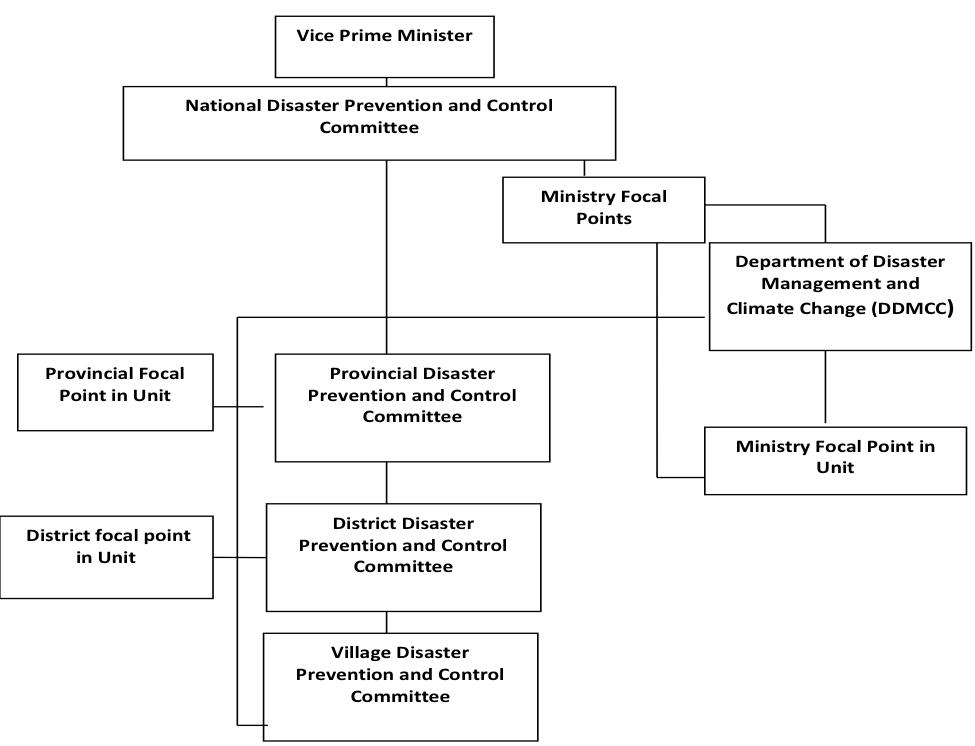
\includegraphics[width = \linewidth]{Figures/laopdr.png}
\end{center}
\end{figure}
   
{\flushleft \large \bfseries Lao Disaster Information System (LaoDi)}

\vspace{0.4 cm}

This initiative aims to strengthen the capacities of Lao PDR to provide information on disaster damage and loss to support national planning and Sendai1 framework. The LaoDi provides authorized users to access disaster data and enables to monitor, analyze vulnerabilities in specific area in Lao PDR and the collected data will be shared with line ministries and stakeholders.

\vspace{0.4 cm}

LaoDi was developed to record, store and analyze loss and damage data in Lao PDR. It was established by DDMCC with technical and financial support from the United Nations Development Programme (UNDP) and the Asian Development Bank (ADB). 

\vspace{0.4 cm}

LaoDi has two modules:  Administration and Analysis Module

\begin{enumerate}
\item Administration Module is designed for authorized user such administrator ora supper user. In this module, the user can (i) manage the database (add, update or delete); (ii) Manage region (provinces, districts and villages); (iii) Manage the  collected data(  delete, modify and updated); (iv) Manage  the maps and (v) Create and manage other users.
\item Analysis Module is for general users to access, the user can (i) analyze the collected data by queries; (ii) identify the  vulnerable area by  province, district  but not yet by villages or by village cluster; (iii) identify the  vulnerable areas by  causes,  type of disasters; and (iv) report  the analyzed result with graphs, tables and maps.
\end{enumerate}

LaoDi data can be exported to Microsoft Excel by statistics and crosstab statistics tools, while data analysis can be made using the chart and thematic map tool. Data analysis can be made at national level, provincial level, district level and village level from selections of query criteria. The LaoDi data is ongoing and will be updated by the Department of Disaster Management and Climate Change (DDMCC), Ministry of Natural Resources and Environment(MONRE). It is open and accessible to the general public at www.laodi.laodisaster.gov.la.

\vspace{0.4 cm}

The LaoDi online application used DesInventar methodology (www.desinventar.net). The database platform and methodology have been implemented in 25 countries in the Asia Pacific region, as well as America, Africa and Europe. LaoDi was established in Lao PDR by DDMCC after a series of consultation workshops between DDMCC officials and UNDP, followed by validation with key line ministries who will be provided data on disaster loss and damage.

\vspace{0.4 cm}

The LaoDi is focuses on direct loss and damage data resulting from natural disasters in Lao PDR, including human life, housing, road agriculture, and education and health sectors. The LaoDi data was collected from provincial disaster management committee (PDMC), district disaster management committees (DDMC), the Ministry of Agriculture and Forestry (MAF), Ministry of Public Works and Transport (MPWT), Ministry of Labor and Social Welfare(MLSW), Ministry of Health (MoH), Ministry of Education, and provincial departments of these line ministries.

\vspace{0.4 cm}

The data of loss and damage from natural disaster are primarily collected from Provincial Disaster Management Committee which also is focal point secretariat. However if the data is not available from PDMC, the data is based on following concerned ministries.

\begin{itemize}
\item Data of human life and housing is collected from Ministry of Labor and Social Welfare(MLSW)
\item Data road sectors is collected from Ministry of Pubic Work and Social Welfare(MPWT)
\item Data of agriculture is collected from Ministry of Agriculture and Forestry(MAF)
\item Data of hospital and health centers is collected from Ministry of Health(MH)
\item Data of schools is collected from Ministry of Education and Sports (MES).
\end{itemize}


{\flushleft \bfseries Current available data in LaoDi is}
\begin{itemize}
\item The  historical data between 1990 and 2012  received from Ministry of Labor and Social Welfare
\item Updated Data: from annual reports of DDMCC between 2014 and 2016.
\item Total of 4448 datacard(records): up to district level  with five main sectors(Agriculture , education, health, labour, and road sectors)
\item Only around 150 road-related data: roads and bridges  data
\item Only 50 data variables (data types): number  of  Deaths people; Injured people; Missing people; Destroyed houses; Destroyed crops; Damaged road; 16 main disaster events; Floods, drought, epitomic, cool wave....
\end{itemize}

{\flushleft \bfseries Expected data for LaoDi is}
\begin{itemize}
\item Direct disaster data  of five main sectors: (i) Agriculture sector; (ii) Education sector; (iii) Health sector; (iv) Labor and social sector and (v) Road sector;
\item Data variables will be more than 170 (e.g number of people deaths, destroyed house,…)
\item Main disaster events are around 20 (Floods, drought, epitomic, cool wave...)
\item The regularly up to-date data  will be received  from provinces via online data entry   and  up to villages level
\end{itemize}

\textbf{LaoDi is still operated offline, but work in Local Area Network (LAN) of the DDMCC office.}

\vspace{0.4 cm}

{\flushleft \bfseries Key Challenges}
\begin{itemize}
\item Lacking human capacity in the area of disaster risk management and emergency responses;
\item Information and data is not yet updated; 
\item Some data and information is not yet available;
\item Local Infrastructure to support geo-based infrastructure is still young; and 
\item Lacking investment.
\end{itemize}

\begin{center}
{(Kob Chai lai lai - Thank you very much) \par}
\vspace{0.5 cm}
\textbf{Keywords:} remote sensing, economic development, challenge, technology independence.
\end{center}

\section{Malaysia}

\vspace{0.5 cm}

{
	\begin{center}
	{\large \bfseries Geospatial Technologies in Malaysian Disaster Planning and Management\par}
	\vspace{0.5 cm}
	{\bfseries Associate Professor Sr Gs Dr Abdul Rashid Mohamed Shariff\par}
	{\itshape University Putra Malaysia\par}
	{\itshape Email: rashidpls@upm.edu.my\par}
	\end{center}
	{\tab The ASEAN Social-Cultural Community (ASCC) Blueprint 2015-20125 is an important step forward in creating a more resilient and self-sustainable community and region. This paper shares the Malaysian approach and hopes the cooperation and ASEAN spirit will lead to the materialization of this highly valued blueprint.
	
\vspace{0.4 cm}

The National Security Council is a Federal agency under the Prime Minister's Department mandated with the responsibility for managing and coordinating the implementation of policies related to the security of Malaysia and providing policies and mechanism for national disaster management and relief. The three core functions of the NSC are defending national sovereignty and strategic importance, crisis and disaster management and border management of land, maritime and air. In order to coordinate government agencies in tackling disasters, the National Disaster Management Agency (NADMA) was set up in 2015 and it coordinates the relevant authorities such as the Malaysian Armed Forces, Police, Malaysian Civil Defence Department, Fire and Rescue Department, Rela, Social Welfare Department and other relevant agencies. NADMA's GIS Centre at Cyberjaya  using the Dashboard Concept is expected to be operationalized in 2018 with Malaysian Space Agency (ANGKASA) providing the geospatial data processing infrastructure and support. The core agencies providing geospatial data for disaster management are Malaysian Metrological Department (MMD), National Survey and Mapping Department (JUPEM), National Remote Sensing Agency (ARSM), National Space Agency (ANGKASA), Malaysian Centre for Geospatial Data Infrastructure (MaCGDI), Public Works Department (JKR), Drainage and Irrigation Department (JPS). In keeping abreast with current developments, low-cost satellites are gaining interest, especially for environmental monitoring, particularly from a state government and university research centres. A framework of cooperation is being formalized for cooperation between Malaysian universities and ANGKASA  on satellite research and development, with a low cost micro-satellite program with Hokkaido/Tohoku university being planned. Research on Deep Learning and artificial intelligence (AI) has made a sound footing at local universities and there is good potential to develop application systems from current research level status. Big data holds a major potential to contribute to disaster management and the role of MacGDI to enable  data sharing and a free flow of data will enhance the useful applications of geospatial data. The national geospatial policy currently being formulated will catalyse this cooperation. The use of high precision satellite positioning will help in getting better mapping and location information for better disaster management decision making. Currently a high precision multi-gnss is being tested at an oil palm plantation with JAXA and collaboration with Keio university, Tokyo university and Universiti Putra Malaysia. The results of such collaboration will not only benefit agriculture but the resulting high accuracy maps can be of aid to disaster management, particularly in flood mitigation. In order to have greater acceptance of technology, the production of simple to operate and beneficial devises become necessary. Internet of Things (IoT) is one example of such developments which has received support of the Malaysian government. Plans are afoot to create an entrepreneurship industry in this field and Malaysian Institute of Microelectronics Systems (MIMOS) has been entrusted with this leadership role. Mimos has created a roadmap for the national IoT strategy (\url{http://mimos.my/iot/National_IoT_Strategic_Roadmap_Summary.pdf}). 
	
\vspace{0.4 cm}
  
The major cost component during the disaster management implementation is the logistics management that can make about 80\% of total cost of a disaster response. It is not only an  issue of cost but the need for timely and efficient coordination as disaster logistics management is currently being handled by multiple government organization with different objectives and stakeholders. Although each agency has a working logistics management system, there is no apparent communication with each other. There is no real-time system on the availability and current location of resources and assets that have been allocated for the purpose. Based on feedback from experienced ground personnel who has been involved in dozens of disaster operations, it was found at the 'de-brief session' that the main problems that exist and need to be addressed is the communications problem. The communication flaws can be contributed by the weaknesses among the personnel, the weaknesses of some agencies standard operating procedures (SOPs), command and order and from the radio emergency communication system itself.
	
\vspace{0.4 cm}
  
	Empowerment of local communities against natural hazards not only renders support to the disaster preventions efforts but when implemented as a WEB GIS, as in the case of Ulu Klang Highlands community, was found to have benefits of helping in the development of a community friendly web GIS based information system, ability to integrate the web site with data from metrological and other relevant sources, empowered the community to upload relevant environment sensitive information and to produce updated maps that can be printed and downloaded by local residents. These brought benefits to the residents as they were able to view and have easy access to the map in the web and other information which are relevant such as rainfall data, can be active players in monitoring their local topography an environment and can link directly to metrological and other external data sources.
		
\vspace{0.4 cm}
  
	Based on the assessment of the current situation, some potential projects that can benefit from the integrated use of the space and geospatial technologies are cross-boundary haze, illegal human trafficking, crowd sourcing information and Illegal land cutting and land clearing.
		
\vspace{0.4 cm}
  
	Although there is ASEAN cooperation and agreement on trans-boundary haze pollution, well integrated and efficiently executed geospatial applications will help in the success of combating trans-boundary haze, especially through effective data sharing procedures. Illegal human trafficking is a problem awaiting a geospatial solution. This activity is directly a geospatial phenomenon as no illegal human trafficking can occur without geographical movement of the victim. The current mobile telephone technology can be an innovative tool in helping trace this illegal human movement. As greater masses of people can exposed to technology the time is ripe to educate and cultivate crowd sourcing data from people on the ground. In the case of Malaysia, just the Civil Defence Agency alone has 1 million people who are their ground volunteers. Tools such as low cost high accuracy multi-gnss receivers will enable these volunteers to supply ground data with very high accuracy. As for land cutting and clearance activities, monitoring and enforcement of illegal and dangerous cutting and clearing of land can help avoid landslides, mud floods and related disasters which have brought catastrophic consequences in the past.
		
\vspace{0.4 cm}
  
In conclusions, it is indisputable that space and geospatial data is a critical requirement in building a resilient society. Use of these data, together with a data infrastructure and data sharing are fundamental  parts of a resilient system. Communication, training and retraining are vital components of capacity building that cannot be overlooked. With the current pace of technological changes, having a society that is up to date, knowledgeable and skilful in the use of the geospatial technology will be an asset to the country and ASEAN region. The wisdom and efficiency in utilizing these geospatial technology will ensure a safe and secure society for generations to come. 

\par}
}


\section{Myanmar}

\vspace{0.5 cm}

	\begin{center}
	{\large \bfseries Presentation Summary by Myanmar on the ERIA Research Project Wrap-up Meeting\par}
	\vspace{0.5 cm}
	{\bfseries Daw Thiri Maung\par}
	{\itshape Ministry of Social Welfare, Relief and Resettlement (Myanmar)\par}
	{\itshape July 6, 2017\par}
	\end{center}
	{\tab Myanmar is prone to the natural disasters and the frequencies and the intensities of the disasters are getting higher.  According to the global reports, the rank for the disaster frequency of Myanmar is 42 out of 171 countries while the rank for the readiness for response to the disaster is 15.
		
\vspace{0.4 cm}
  
After the catastrophic cyclone Nargis in 2008 which triggered the 21\% total damage and loss of GDP in 2007 fiscal year, Myanmar has made emphasis to the Disaster Risk Reduction in momentum. The country bears average annual loss of about 3\% of GDP due to the natural disaster. In 2015, it also suffered the nation-wide flood and severe landslide in the mountainous regions especially in the Western part of the country and these happened 3.1\% total damage and loss of GDP. The Government of Myanmar has laid down its development vision to be 'A developed nation (middle income country) that is integrated into the global community' in its National Comprehensive Development Plan (NCDP), 2030. A disaster can draw back the development gains and can interrupt the development and sustainability of the country. In this regards, to achieve the resilient development in Myanmar, the National Disaster Management Committee (NDMC) has been comprised and chaired by the Vice President of the Government of the Union of Myanmar aiming to promote the Disaster Management System in Myanmar in line with global and regional frameworks. 
		
\vspace{0.4 cm}
  
The NDMC is the highest decision making body and 12 working committees has been composed under the supervision of the NDMC. Relief and Resettlement Department (RRD) of the Ministry of Social Welfare, Relief and Resettlement is the focal department for the Disaster Management. Myanmar also enacted the Disaster Management Law (2013) and the Disaster Management Rules (2015) as law enforcement is necessary to ensure the sustainable development while carrying out the disaster risk reduction and management activities without any interruption. Moreover, Myanmar Government developed the Myanmar Action Plans on Disaster Risk Reduction-MAPDRR (2012) and now MAPDRR is under revision in line with SFDRR, SDGs and other regional and global concerned frameworks.
		
\vspace{0.4 cm}
  
Based on the experience and lesson-learnt from the previous MAPDRR (2012), the new MAPDRR (2017) will be comprised with four main areas and one of them is "Assessing disaster and extreme events risk and creating public awareness on DRR in Myanmar" and there will be 8 priority actions for risk reduction by mainly applying the space-based and geospatial  technologies. 
		
\vspace{0.4 cm}
  
Since 2012, Myanmar has started to upgrade its disaster management system by utilizing advanced technology like space technology and received the Technical Advisory Mission (TAM) of the UNSPIDER of UNOOSA. The TAM provided the recommendations to utilize the space technology widely in the disaster management. Myanmar Government has understand that the advanced and techanical based disaster management mechanism has become the crucial and necessary requirement for attempting to have the resilient community to the natural disaster and sustainable development and RRD reformed its organization structure by means of the establishment of the Emergency Operations Centre (EOC) as one of the operating organs of RRD in 2013. EOC has been comprised with four different units including the technical unit for handling the space-based and geospatial information. This technical unit is still under nurturing stage for the human resource development to get fully functioning for analysing the satellite imageries and perform the researches on the risk analysis to contribute for the disaster management activities. It is still necessary to get the capacity development measures for the technical skills improvement and experiences as well.
		
\vspace{0.4 cm}
  
Myanmar also tried to be a member to the International communities for utilization of space technology in disaster emergency and disaster management and already got the technical assistance and data and information in disaster emergency from the Sentinel Asia and the International Charter. Being a member to the Asian Disaster Reduction Centre (ADRC), Myanmar has the rights to request to the Sentinel Asia. Moreover, Relief and Resettlement Department (RRD), the National Disaster Management Organization (NDMO) has become the Authorized User of the International Charter to get the speedy activation process. Besides, Myanmar has another option for accessing the Space technology that is the Procedural guidelines on "Utilization of Earth observation data during emergency response" developed for ASEAN group.
		
\vspace{0.4 cm}
  
Furthermore, RRD is tried to allocate the budget for purchasing the high resolution satellite imageries in the future fiscal year for having the chance to utilize the satellite imageries in the relocation stage after some disaster emergencies and risk assessment measures when it is necessary to provide the said images. In addition, the training course for the Geoinformatics Applications in Disaster Management was developed and this course is used to deliver in the Disaster Management Training Centre (DMTC) of RRD to the government officials and staffs who are responsible to the disaster management in Myanmar. The objective of the training is to "raise awareness amongst the participants and develop basic skills for effectively utilising the Geographic Information Systems and RS/ space based information in Disaster Management". This course is comprised with 4 modules, namely; Disaster Management Terminologies and Concepts, Introduction to GIS, Remote Sensing, GPS and Internet Mapping Services, Geoinformatics for Mapping and monitoring of Hazards, Vulnerability and Risk Assessment and Geoinformatics for Disaster Management Planning and Emergency Response.
		
\vspace{0.4 cm}
  
Disaster risk reduction and disaster management is the cross-cutting issue and it is very crucial for the national development and sustainability. In order to ensure the sustainable development, it is vital to be disaster resilient and the disaster risk reduction measures are critical to make the best use of space-based and geospatial technologies. Moreover, it is important to dessiminate the results and products acquired from these technologies not only to the concerned agencies to have the practice to utilize in their routine works in DRR but also to the communities for their awareness raising. Exchanging the knowledges and best practices on utilization of space-based and geospatial technologies through the regional and global meetings and workshops are very helpful to widely utilze and apply the technologies in the field of disaster management.
\par}


\section{Philippines}

\vspace{0.5 cm}

	\begin{center}
	{\large \bfseries Disaster Risk Reduction and Management (DRRM) in the Philippines and the Southeast Asian Region through 
Space Technology\par}
	\vspace{0.5 cm}
	{\bfseries Adrian Josele G. Quional\par}
	{\itshape National SPACE Development Program\par}
	{\itshape 37th Flr. LKG Tower, 6801 Ayala Ave., Makati City, 1226 Philippines\par}
	\end{center}
	{\tab The Philippines is located near the equator and along the Pacific Ring of Fire which makes it vulnerable to natural disasters such as typhoons, earthquakes, and volcanic eruptions, endangering the natural resources and biodiversity endowed to the country. A notable major disaster that struck the Philippines is Typhoon Haiyan (local name: Typhoon Yolanda) on November 2013 which brought an estimated cost of damages worth PHP 89.6 billion (USD 1.77 billion), with 6,300 deaths and 1,081 gone missing. This scenario is a major concern for the Philippines and measures needed to be adapted given that a similar disaster is possible to happen in the future due to the Philippines' location. An effective Disaster Risk Reduction and Management (DRRM) measure that can be taken by the country is the use of space technology, particularly satellite technology.
		
\vspace{0.4 cm}
  
The country is gradually emerging as a space-faring nation, as evidenced by the continuous space development efforts throughout the past years. Looking ahead, the Philippines, through the National Space Promotion, Awareness, and Capabilities Enhancement (SPACE) Development Program (or NSDP), developed strategic roadmaps for the future space program of the country. Among these roadmaps includes the Satellite Development Roadmap which contains the satellite requirements of the Philippines for the next 15 years. Particularly, satellite technology for the Philippines would bring enormous benefits for the country, particularly on applications for national security, agriculture, and disaster management. While all of the satellites being planned by the Philippines have a direct or indirect application for disaster management (in terms of communications and Earth observation applications), there are particular satellites that has the greatest contribution to this use. In particular, planned satellites that have immense applications for disaster management includes a Synthetic Aperture Radar (SAR) satellite and a Microwave Satellite for Precipitation Monitoring. 
		
\vspace{0.4 cm}
  
The coupled use of a SAR and a Microwave Satellite can greatly enhance DRRM efforts throughout the country. By measuring precipitation and rainfall using a Microwave Satellite, combined with the data from the SAR satellite, comprehensive results can be timely distributed to various decision and policy makers in critical times of disasters; thereby enhancing humanitarian aid for the affected areas.
		
\vspace{0.4 cm}
  
Given this strategic plan of the country to develop satellites for disaster management, the Philippines can lead the way for the Southeast Asian Region, being in a prominent location for typhoons and disasters. As the country is strategically located between the Pacific Ocean and the mainland Southeast Asia, the path of typhoons mostly cross the Philippine archipelago onto either East Asia or Southeast Asia, making the country, indeed, at the forefront of typhoons. Therefore, being at the frontlines of Southeast Asia in terms of typhoons, an effective utilization of satellite technology for disaster management in the country would help the whole region as it would reduce the risk of disaster for the other countries. An "ASEAN Satellite Constellation" of SAR and/or Microwave Satellites would prove a valuable asset for the region as it would mean a greater regional coverage.
		
\vspace{0.4 cm}
  
However, physical infrastructure for satellite technology would not be effective without satellite information sharing. Thus, there is a need for the countries in the region to engage in satellite information sharing to promote inter-operability and interconnectivity throughout the region in terms of satellite technology. A Satellite Data Sharing Policy for the Southeast Asian Region for disaster management, amenable to each country's policies and not endangering the security of each nation, would prove useful.
		
\vspace{0.4 cm}
  
Lastly, a Regional Center for Water Information can be established in the Philippines to pool in researchers and technologists from Southeast Asia and to facilitate satellite data sharing among countries. This Regional Center can be the centerpiece in Southeast Asia in terms of utilizing water information, in this case for disaster management. 
		
\vspace{0.4 cm}
  
The Philippines has been at the forefront of disasters and typhoons in Southeast Asia, as manifested by the recent Typhoon Haiyan that struck the Philippines on 2013, where no other typhoon to date matches the devastation brought upon by it. With the Philippines slowly emerging as a space-faring nation, crafted plans for its future space program, the development and utilization of various satellites for disaster management is included at the forefront of its strategy. The use of a SAR and Microwave Satellite, not only in the Philippines but also for the whole Southeast Asia, would be a valuable asset. A Satellite Data Sharing Policy for the region should also be discussed upon in order to effectively utilize the satellite data. Lastly, a Regional Center for Water Information can be established in the Philippines which would play a vital role in the region in the facilitation of water information and research. 
\par}

\section{Thailand}

\vspace{0.5 cm}

{
	\begin{center}
	{\large \bfseries Thailand Disaster Risk Manage utilized Space Technology\par}
	\vspace{0.5 cm}
	{\bfseries Jakrapong  Tawala\par}
	{\itshape Geoinfomatics and outreach scientist\par}
	{\itshape Geo-informatics and Space Technology Agency (Public Organization)\par}
	{\itshape 196 Phahonyothin Rd., Ladyao, Chatuchak, Bangkok, THAILAND\par}
	{\itshape jakrapong@gistda.or.th\par}
	\end{center}
	{\tab Thailand is less susceptible to natural hazards than many of the countries in the Asia – Pacific. Geography and location of Thailand help insulate the country from many of the impact of metrological and geophysical natural disasters. However, Thailand is agricultural industry and highly development urban areas leave large portions of the population and the economy vulnerable to disasters such as flooding, drought, landslides and forest fire. 
	
\vspace{0.4 cm}

Over the past two decades, space technology has become a significant part of our daily lives and can play important roles in the disasters risk reduction and management. Thailand has been involved in satellite remote sensing since the launch of NASA ERTS-1 Programme in 1971 through Thailand Remote Sensing Programme (TRSP) under the National Research Council of Thailand (NRCT). In 2000, Geo-Informatics and Space Technology Development Agency (Public Organization): GISTDA was established in order to enhance the utilization in remote sensing and GIS and responsibilities the activities for space technology applications in Thailand particularly for disaster management. Thailand Monitoring System (TMS) was initiated by GISTDA to cope and monitor disaster and daily on-line publish analytic geo-information from satellite imagery for related organization and private sector. The system includes flood, drought and forest fire and can be accessed at tms.gistda.or.th.

\vspace{0.4 cm}

Flooding is the most serious hazard in Thailand and every part of the country struggles with flood-related damages annually.  During monsoon season in Thailand, GISTDA monitors flood situation and agricultural areas in Thailand every 7 days utilized RADARSAT data to monitor agricultural areas and evaluate damaged zones for general areas and Cosmo-skymed data to monitor critical areas due to its constellation capability (4 satellites). Rain cloud information from COMS satellite is available in hourly, daily, weekly and monthly. These information are served to the government and published via web service (flood.gistda.or.th)

\vspace{0.4 cm}

Drought is an increasingly serious hazard for parts of central and eastern of Thailand. Drought conditions are most common from January through May and are alleviated by the onset of monsoon season. GISTDA use a set of MODIS data (7 days) to calculate drought indices, Normalized Difference Vegetation Index: NDVI and Normalized Difference Water Index: NDWI, for drought risk area assessment and weekly published on http://drought.gistda.or.th. This information is necessary for the government to warn and assist the farmer. Moreover, surface water database from Landsat satellite image has been collected for drought monitoring as it is an indicator of water shortage. GISTDA also developed Field Server Ground Station to automatics collect field data such as humidity, soil moisture, rain volume and crop growing etc. This data will be integrated with satellite data for precise data from the field. Currently, there are 25 stations was installed spread the whole country in difference crop type. 

\vspace{0.4 cm}

Forest Fire annually occurs during the dry season from December to May with their peak in February-March. Fires, Mostly classified as surface fires, mainly take place in; Mixed Deciduous Forest, Dry Dipterocarp Forest, and Forest Plantations, and to some extent in Dry Evergreen Forest, Hill Evergreen Forest or event in some parts of the Tropical Rain Forest. These surface fires consume surface litter, other loose debris on the forest floor and small vegetation. In Thailand, forest fire is daily report TMS system (fire.gistda.or.th) publishing daily hotspots utilized TERRA/AQUA-MODIS data, haze, smoke. GISTDA weekly generates wildfire risk area analyzed from hotspots accumulated 10 years , land-use, burnt NDWI area and weather to predict trend of fire in each year. Burnt area every 16 days also extracted using LANDSAT- 8 satellite image. Beside, GISTDA established GISTDA Forest Fire and Smoke Operation Center in 9 provinces in northern of Thailand where forest fire is common issue.   In this center will received product of remote sensing and GIS data from GISTDA to support forest fire management and training of data interpretation and effectively using form GISTDA experts. Currently, GISTDA receives daily hotspot data from SUOMI-NPP satellite (2 time/day) integrate with MODIS data. By doing this, Thailand will have more detail information of forest fire and number of hot spot may significantly increase because number of round and resolution of satellite. Mobile Application for alert and report the situation in the fire area was developed to get more precise fire location data. 

\vspace{0.4 cm}

Base on GISTDA experiences, space technology still remain plays important roles for disaster management in every state of disaster situation in the future.  Satellite image gives the overview information of disaster situation which necessary for understanding, management and decision making. Precise location information form constellation of GNSS will lead you to exact location to rescue and assist on time. Right information integrate with appropriated management processing and new technology will result rapid resolved situation for example hot spot situation in northern part of Thailand has continued to decline in every year because of management in the right point and location with understanding the situation utilized information from space technology. 
\par}
\begin{center}
\textbf{Keywords:} space, technology, natural disasters, Thailand \par
\end{center}
}

\section{Vietnam}

\vspace{0.5 cm}

	\begin{center}
	{\large \bfseries Potential of GeoSpatial/Space -- Based Service in Vietnam\par}
	\vspace{0.5 cm}
	{\bfseries Dr. Vu Anh TUAN\par}
	{\itshape Vietnam National Satellite Center\par}
	\end{center}
	{\tab The 2016 World Disaster Report showed that Vietnam has been one of five countries most affected by the natural disaster and climate change in the world. In the last 10 years, according to MONRE (Ministry of Natural Resource and Environment), there are around 500 deceases, damage of 1.5\% of GDP per year cause by disasters. There are many type of disaster in Vietnam.  The top five high frequency disasters are: Flooding; Storm; Draught; Flash Flooding; Erosion/sedimentation.
	
	
Using Space-based service for disaster management in Vietnam is currently issues by research institutions as well as management agencies. Recently, Vietnam is building up an infrastructure for geospatial data called Vietnam Data Cube. This will be open-sharing system for all available geospatial data of Vietnam, including free satellite data such as Landsat, MODIS, Sentinel; Vietnam's satellite data (VNREDSat 1; LOTUSat 1 and 2) and other data. The Vietnam Data Cube is being built based on the Data cube (http://ceos-cube.org/). The Vietnam Data Cube will provide ability of ease of use and access to space-based data with multiple dataset interoperability and spatial consistency. It is also combined with built-in data processing algorithm and API which can be used for "Analysis Ready" of data products for all users. The Vietnam Data Cube is planned to be launched in January 2018 with two demonstrate applications: Forest monitoring and Water quality monitoring. Since the open of space-based data and service of Vietnam Data Cube, it can be considered for nominee of space-based service for disaster management in Vietnam as well as in ASEAN countries. However, toward a space-based service for disaster management, the investment issues need to be clarified are: infrastructure (Data Cube – based); Data system (Data Cube similar); Software; Trained professionals and Web-based services system. This system will help ASEAN countries to share common understanding, EO and GeoSpatial data and help people in early warning; rescue information.
\par}


\singlespacing
%next line adds the Bibliography to the contents page
\addcontentsline{toc}{chapter}{Bibliography}
\bibliography{biblio} %use a bibtex bibliography file
\bibliographystyle{plain}  %use the plain bibliography style


\end{CJK}
\end{document}

